%Kompiliuoti su XeLaTeX ir BibTeX

\documentclass[a4paper, 12pt, oneside]{article}

\usepackage[yyyymmdd]{datetime}

\usepackage{fontspec}
\usepackage{fontenc}
\usepackage{ulem}
\usepackage{cite}
\usepackage{mathtools}
\usepackage{amsmath}
\usepackage{amssymb}
%\usepackage{float}
\usepackage{graphicx}
\usepackage{multirow}
\usepackage[hyphens]{url}
\usepackage{caption}
\usepackage{subcaption}
\usepackage[svgnames]{xcolor}
\usepackage{lineno}
\usepackage[lithuanian]{babel}
\usepackage{hyperref}
\usepackage{siunitx}
\usepackage{floatrow}
\usepackage{indentfirst}
%\usepackage[parfill]{parskip}

\floatsetup[table]{capposition=top}

\hypersetup{breaklinks=true}
\urlstyle{same}

\usepackage{geometry}
\pagestyle{myheadings}
\geometry{
	left=3cm,
	right=1cm,
	top=2cm,
	bottom=2cm,
}
\pagenumbering{arabic}
\linespread{1.25}

\graphicspath{ {images/} }

\renewcommand{\dateseparator}{-}
\addto\captionslithuanian{\renewcommand{\figurename}{pav}}
\addto\captionslithuanian{\renewcommand{\refname}{6 \hspace{0.1cm} Naudotos literatūros sąrašas}}
\addto\captionslithuanian{\renewcommand{\tablename}{lentelė}}

\DeclareCaptionLabelFormat{numfirst}{#2~#1}
\captionsetup[figure]{labelformat = numfirst, labelsep = period}
\captionsetup[table]{labelformat = numfirst, labelsep = period}

\newcommand{\textblue}[1]{{\color{Blue}#1}}
\newcommand{\textred}[1]{{\color{Red}#1}}
\newcommand{\comment}[1]{\newline\textblue{#1}\newline}
\newcommand{\commentNL}[1]{\textblue{#1}\newline}
\newcommand{\commentMA}[1]{\textred{#1}\newline}
\newcommand{\ttt}[1]{\texttt{#1}}
\newcommand{\pT}{p_{\mathrm{T}}}
\newcommand{\ET}{E_{\mathrm{T}}}
\newcommand{\WW}{W\! W}
\newcommand{\ZZ}{Z\! Z}
\newcommand{\WZ}{W\! Z}
\newcommand{\tbarW}{\bar{t}W}
\newcommand{\ttbar}{t\bar{t}}
\newcommand{\emu}{e\mu}
\newcommand{\mumu}{\mu\mu}
\newcommand{\gJets}{\gamma\! +\!\mathrm{Jets}}
\newcommand{\WJets}{W\! +\!\mathrm{Jets}}
\newcommand{\dtW}{tW\! + \! \bar{t}W}
\newcommand{\DYee}{\mathrm{DY} \! \rightarrow \! ee}
\newcommand{\DYmumu}{\mathrm{DY} \! \rightarrow \! \mu\mu}
\newcommand{\DYtau}{\mathrm{DY} \! \rightarrow \! \tau\tau}
\newcommand{\DY}{\mathrm{DY}}
\newcommand{\ltq}[1]{{\quotedblbase{}#1\textquotedblleft{}}}
\newcommand{\Lumi}{{\cal L}_\mathrm{int}}
\newcommand{\invfb}{fb$^{-1}\,$}
\newcommand{\invpb}{pb$^{-1}\,$}
\newcommand{\QCD}{QC\! D}

\newlength\q
\setlength\q{\dimexpr .5\textwidth -2\tabcolsep}

\hyphenation{eks-pe-ri-men-tą}
\hyphenation{so-le-noi-das}
\hyphenation{Feinmano}
\hyphenation{ha-dro-no}
\hyphenation{MadGraph}
\hyphenation{už-re-gis-truo-tų}
\hyphenation{miu-o-nų}
\hyphenation{in-te-gruo-tą-jį}

\begin{document}
%\linenumbers

\begin{titlepage}
\centering
{\large Vilniaus universitetas \\ Fizikos fakultetas \\ Teorinės fizikos ir astronomijos institutas \par}
\vspace{3.5cm}
{\Large Marijus Ambrozas \par}
\vspace{0.3cm}
{\Large Drell-Yan proceso triukšmo įvykių skaičiaus įvertinimas klaidingo atpažinimo metodu\par}
\vspace{0.8cm}
{\large Magistrantūros studijų mokslo tiriamasis darbas \par}
\vspace{0.8cm}
{\large Teorinės fizikos ir astrofizikos \\ studijų programa \par}
\vspace{3.5cm}
{\large \begin{tabular*}{0.9\textwidth}{@{\extracolsep{\fill}}ll}
Studentas & Marijus Ambrozas\tabularnewline[0.5cm]
Darbo vadovas & dr.\ Andrius Juodagalvis\tabularnewline[0.5cm]
Instituto atstovas & prof.\ Egidijus Anisimovas\tabularnewline[0.5cm]
\end{tabular*} \par}
\vspace{4cm}
{\large Vilnius $2020$\par}
\end{titlepage}


\clearpage
\addtocounter{page}{1}
\addtocontents{toc}{\protect\setcounter{tocdepth}{2}}
\tableofcontents
\clearpage

\section{Įvadas}% \addcontentsline{toc}{section}{Įvadas}

Didelių energijų fizikoje protonas aprašomas naudojantis R.\ Feinmano pasiūlytu partonų modeliu \cite{FeynPartons},
pagal kurį protono sandarą galima nusakyti naudojantis partonų pasiskirstymo funkcijomis \cite{BjorkPartons}.
Norint geriau suprasti procesus, vykstančius protonų susidūrimų metu, svarbu partonų pasiskirstymus žinoti kuo tiksliau.
Kvantinės chromodinamikos (angl.\ \textit{quantum chromodynamics} -- QCD) teorija nenumato partonų pasiskirstymo funkcijų parametrų.
Jie gaunami funkcijas pritaikant prie eksperimentinių tyrimų rezultatų \cite{NNPDF, PDF_ABMP16, CTEQ2019}.

Protonams susiduriant su didžiule energija kvarkas iš vieno protono ir antikvarkas iš kito gali anihiliuoti
ir sukurti leptono-antileptono porą.
Toks procesas vadinamas Drell-Yan procesu \cite{DYoriginal}.
Didelio tikslumo naujausių Drell-Yan proceso diferencialinio reakcijos skerspjūvio eksperimentinių matavimų
rezultatai \cite{DY2013, DY7TeVatlas, DY2015, DY8TeVatlas, DY2019} pasitarnauja partonų pasiskirstymo funkcijų
tikslinimui, teorinių modelių bei jų perturbatyvinių pataisų testavimui.
Drell-Yan proceso tyrimo rezultatai yra svarbūs ir kituose eksperimentiniuose didelių energijų fizikos
tyrimuose, kuriuose Drell-Yan procesas yra dominuojantis triukšmas \cite{Higgs2018, Zprime, SUSYtau}.
Taigi, Drell-Yan procesas yra vienas iš  kertinių tyrimo objektų eksperimentinėje dalelių fizikoje.

CERN Didžiajame hadronų greitintuve (angl.\ \textit{Large Hadron Collider} -- LHC) kas $25$ ns vyksta $13$ TeV
energijos protonų susidūrimai \cite{LHC_13TeV_25ns}.
Kartais susidūrimų metu sukuriamos masyvios nestabilios dalelės (pvz., $Z$ bozonas, Higso bozonas ir pan.),
kurių vidutinė gyvavimo trukmė yra labai trumpa.
Aplink protonų susidūrimo vietas išdėstytais dalelių detektoriais įmanoma užregistruoti tik tokių
dalelių skilimo produktus: fotonus, elektronus, įvairius hadronus bei miuonus.
Įvykiai, kurių metu detektoriuje užfiksuojama leptono-antileptono pora vadinami Drell-Yan proceso įvykio kandidatais.
Vis dėlto, niekada tiksliai nežinome ar įvykio kandidatas tikrai yra mus dominantis (Drell-Yan signalo) įvykis.
Egzistuoja ir triukšmo įvykiai, kurių galutinis produktas atrodo labai panašiai į galutinį Drell-Yan proceso produktą.
Į triukšmų indėlį reikia atsižvelgti statistiškai įvertinant, kokią dalį visų įvykių kandidatų jie galėjo sudaryti.
Triukšmo įvykių skaičių galima būtų įvertinti naudojant vien tik modeliuotus duomenų rinkinius, tačiau jie turi
netikslumų, į kuriuos visus atsižvelgti būtų labai sudėtinga.
Siekiant tikslesnės detektoriaus išmatuotų pasiskirstymų interpretacijos yra naudojami matavimu grįsti metodai.
Klaidingo atpažinimo metodas, kuris buvo naudojamas šiame darbe, yra taikomas norint įvertinti skaičių tokių triukšmo
įvykių, kurių metu susidariusios hadronų čiurkšlės buvo klaidingai atpažintos kaip leptonai.


\textbf{Šio darbo tikslas} -- įvertinti Drell-Yan proceso triukšmo įvykių skaičių objekto klaidingo atpažinimo metodu.
Tikslui pasiekti iškelti tokie \textbf{uždaviniai}:
1) Įvertinti tikimybę, kad čiurkšlė bus klaidingai atpažinta kaip miuonas;
2) Pritaikant klaidingo atpažinimo tikimybės įvertį nustatyti, kiek Drell-Yan proceso triukšmo įvykių yra susiję su
klaidingai atpažintomis čiurkšlėmis;
3) Įvertinti gauto rezultato statistines ir sistemines paklaidas.
Darbas buvo atliktas naudojant CERN CMS eksperimento 2016 metais užregistruotus protonų susidūrimų duomenis.

\section{Drell-Yan procesas}

Kvantinė chromodinamika aprašo sąveiką tarp hadronus sudarančių dalelių: kvarkų ir gliuonų.
Kasdienėje aplinkoje, kur bendru atveju dalelių tarpusavio sąveikos energijos yra labai mažos,
stipriosios sąveikos konstanta $\alpha_s$ yra labai didelė.
Dėl šios priežasties kvantinių laukų teorijoje naudojamas perturbatyvusis aprašymas žemų energijų stipriesiems procesams
yra netinkamas.
Vis dėlto, stiprioji sąveika pasižymi asimptotine laisve -- reakcijos energijai augant į begalybę, sąveikos konstanta
gęsta ir dalelės sąveikauja vis silpniau \cite{AFreedom}.
Dėl šios savybės šiuolaikiniuose dalelių greitintuvuose vykstančiuose susidūrimuose, kuriuose protonų susidūrimo energija
siekia net iki $13$~TeV, stipriosios sąveikos konstanta tampa pakankamai maža, kad perturbatyvioji kvantinės chromodinamikos
teorija būtų tinkama vykstančių procesų aprašymui.
Pavyzdžiui, sąveikos tarp susiduriančių protonų sudedamųjų dalių -- kvarkų -- energijai siekiant $Z$ bozono masę ($91.2$~GeV),
stipriosios sąveikos konstanta jau turi vertę, siekiančią vos $0.115$ \cite{PDF_ABMP16}.

Norint teoriškai aprašyti hadronų susidūrimus svarbu žinoti, su kokiomis tikimybėmis gali sąveikauti konkrečios
hadrono viduje esančios dalelės.
Šiam tikslui yra naudojamas R.~Feinmano pasiūlytas artinys, vadinamas partonų modeliu \cite{FeynPartons}:
kadangi perturbatyvioji kvantinė chromodinamika yra tinkama tik kai susidūrimų energijos pakankamai didelės,
galima sakyti, kad prie tokių energijų hadrono sudedamųjų dalių -- partonų -- impulso dedamosios, statmenos paties
hadrono judėjimo krypčiai yra nykstamai mažos, lyginant su lygiagrečia hadrono judėjimui impulso dedamąja.
Tai reikštų, kad su hadronu susiduriančios dalelės atskaitos sistemoje jį įsivaizduojame kaip plokščią nejudančių
taškų rinkinį.
Toks artinys atitiktų realybę, jeigu hadrono impulsas būtų begalinis.
Pritaikius šį artinį hadroną galima aprašyti kaip tikimybės tankių rinkinį: kiekvienas tikimybės tankis nusakytų tikėtinumą
aptikti konkretų partoną (kvarką arba gliuoną), nešantį tam tikrą procentinę hadrono impulso dalį $x$ \cite{BjorkPartons}.
Šie tikimybės tankiai vadinami partonų pasiskirstymo funkcijomis.
Partonų pasiskirstymo funkcija $f_{i}(x, Q^{2})$ aprašo tikimybę aptikti protono impulso
dalį $x$ nešantį $i$ tipo partoną (pavyzdžiui, kylantįjį kvarką -- $u$, krentantįjį
kvarką -- $d$ ir t.t.), kai \textit{kietojo} susidūrimo energija lygi $Q$.
Kietasis susidūrimas (angl.\ \textit{hard interaction}) -- procesas, kurio metu vyksta energijos pernaša, palyginama
su pilnąja sistemos energija.
Du partonų pasiskirstymo funkcijų pavyzdžiai, esant skirtingoms susidūrimų energijoms, yra pateikti
\ref{fig:PDFs} paveiksle.

Hadronų susidūrimų metu vykstančių reakcijų skerspjūviai yra apskaičiuojami kaip partonų pasiskirstymo
funkcijų ir partonų tarpusavio reakcijos skerspjūvio kombinacija:
\begin{equation}
	\sigma = \sum_{i, j} \int \mathrm{d}x_1 \int \mathrm{d}x_2 \,
	f_{i}(x_1, \, Q^2) \, f_{j}(x_2 \, Q^2) \, \hat{\sigma}(x_1 p_1, \, x_2 p_2, \, Q^2) \; \mathrm{,}
	\label{eq:PDFxsec}
\end{equation}
čia $\sigma$ -- reakcijos skerspjūvis, $i$, $j$ -- sąveikaujantys partonai, nešantys protonų impulsų $p_1$ ir $p_2$
dalis $x_1$ ir $x_2$, o $f_{i}(x_1, \, Q^2)$ ir $f_{j}(x_2, \, Q^2)$ -- partonų pasiskirstymo funkcijos, kai
energijos pernaša reakcijos metu lygi $Q$.

\begin{figure}[t]
	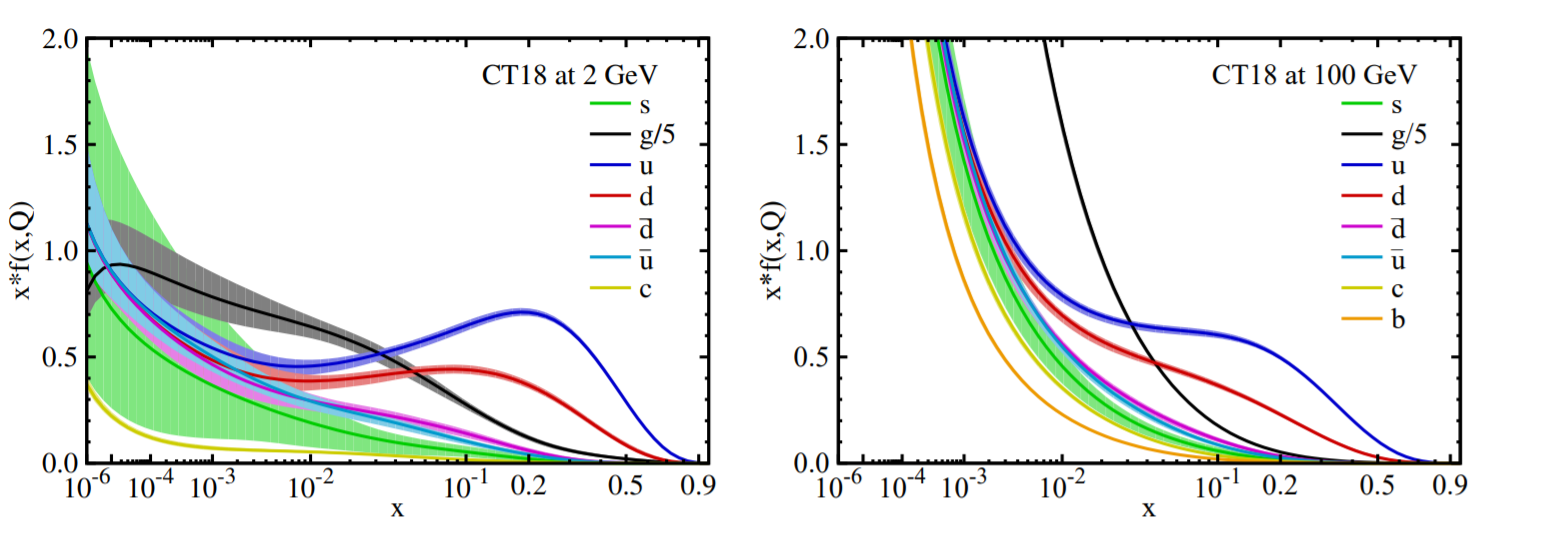
\includegraphics[width=\linewidth]{CT18_PDF.png}
	\caption{\label{fig:PDFs}
		CTEQ-TEA kolektyvo pateikiamos protono partonų pasiskirstymo funkcijos esant skirtingoms susidūrimų energijoms \cite{CTEQ2019}.
		Kairėje -- $Q=2 \; \mathrm{GeV}$, dešinėje -- $Q=100 \; \mathrm{GeV}$.
		Ant horizontalios ašies vaizduojama protono impulso dalis $x$, o ant vertikalios -- tikimybės tankio $f(x,\, Q^2)$
		ir $x$ sandauga.}
\end{figure}


Kvantinės chromodinamikos teorija nenumato partonų pasiskirstymo funkcijų parametrų.
Jie gaunami funkcijas pritaikant prie eksperimentinių tyrimų rezultatų \cite{NNPDF, PDF_ABMP16, CTEQ2019}.
Vieni svarbiausių rezultatų, naudojamų partonų pasiskirstymo funkcijų parametrų nustatymui atkeliauja iš elektrono-protono
sklaidos eksperimentų (anksčiau tokius susidūrimus vykdydavo HERA dalelių greitintuvas Hamburge) bei iš
Drell-Yan proceso, viršūninių kvarkų poros sukūrimo bei vienos čiurkšlės įvykių, kurie vyksta protonų priešpriešinių susidūrimų
metu, tyrimų \cite{CTEQ2019}.

\textbf{Drell-Yan procesas} \cite{DYoriginal} -- tai toks procesas, kai protonų susidūrimo metu anihiliavus kvarkui ir antikvarkui
sukuriama leptono ir antileptono pora.
Šis procesas vyksta apsikeičiant $Z$ bozonu arba virtualiu fotonu per s-kanalą:

\begin{equation*}
	q\bar{q} \rightarrow Z/ \gamma^{*} \rightarrow l^{+}l^{-} \; ,
\end{equation*}
čia $q$ ir $\bar{q}$ žymi atitinkamai kvarką ir antikvarką, $\gamma^*$ žymi virtualų fotoną, o $l^+$ ir $l^-$ -- atitinkamai
antileptoną ir leptoną.
Šią reakciją toliau žymėsime $\DY \! \rightarrow \! l^{+}l^{-}$.
Skirtingos Drell-Yan proceso galutinės būsenos, priklausomai nuo to, kokios rūšies leptonai susidaro, yra
vadinamos kanalais: elektronų kanalas, miuonų kanalas, taonų kanalas.
Kadangi taonai gyvuoja labai trumpai, jų kanalo tyrimas yra sudėtingesnis ir dažniausiai yra vykdomas atskirai,
o tuo tarpu elektronų ir miuonų kanalo tyrimus neretai vykdo ta pati mokslinė grupė.

Drell-Yan procesas tapo svarbiu tyrimo objektu nuo pat pirmojo jo aprašymo $1970$-aisiais
metais, kai S.~D.~Drell ir T.~M.~Yan bandė apibūdinti leptonų ir antileptonų porų susidarymą
hadronų susidūrimų metu \cite{DYoriginal}.
Drell-Yan procesas pirmą kartą eksperimentiškai buvo stebėtas dar tais pačiais metais protonų susidūrimuose
su urano branduoliais \cite{DY_firstExp}.
Šio proceso tyrimas svarbus todėl, kad jame dalyvauja nevalentinis protono kvarkas.
Tai leidžia padaryti svarbių įžvalgų apie protono sandarą.

Šiais laikais teoretikai Drell-Yan procesą gali sėkmingai apskaičiuoti iki trečios eilės
kvantinės chromodinamikos perturbacijų tikslumo (angl.\ \textit{next-to-next-to-leading order} -- NNLO --
reiškia dviejų kilpų ir dviejų dalelių išspinduliavimo pataisas).
Tokios aukštos eilės elektrosilpnosios pataisos nenaudojamos, nes kiekvienos elektrosilpnosios viršūnės
indėlis į reakcijos skerspjūvį yra $>10$ kartų mažiau reikšmingas, lyginant su stipriosios sąveikos viršūne.
Drell-Yan proceso pirmos eilės (angl.\ \textit{leading order} -- LO -- reiškia medžio lygmenį) Feinmano diagramos
yra pavaizduotos \ref{fig:DYfeyn}~pav.

\begin{figure}[t]
\centering
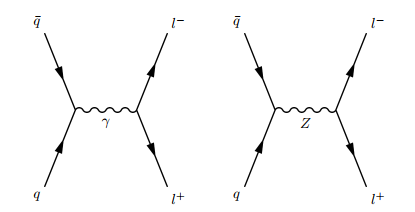
\includegraphics[scale=0.75]{DYprocess.PNG}
\caption{Drell-Yan procesą apibūdinančios medžio lygmens Feinmano diagramos.}
\label{fig:DYfeyn}
\end{figure}


Didelio tikslumo eksperimentiniai Drell-Yan proceso diferencialinio skerspjūvio matavimai \cite{DY2013, DY7TeVatlas, DY2015, DY8TeVatlas, DY2019}
naudojami ne tik partonų pasiskirstymo funkcijoms tikslinti, bet taip pat ir perturbatyviosios kvantinės
chromodinamikos bei elektrosilpnosios sąveikos teorijoms tikrinti.
Be to, šis procesas yra vienu iš pagrindinių triukšmo procesų įvairiuose kituose didelių energijų fizikos tyrimuose,
pavyzdžiui, Higso bozono tyrime \cite{Higgs2018}, ne standartinio modelio dalelės -- $Z'$ bozono -- paieškoje \cite{Zprime},
supersimetrijos paieškoje \cite{SUSYtau} ir pan.
Taigi, tikslūs Drell-Yan proceso matavimai įvairiapusiškai prisideda prie kitų didelių energijų
fizikos tyrimų rezultatų kokybės.


\section{Drell-Yan proceso tyrimo metodika}

Šiame skyriuje pristatomas CERN CMS detektorius bei pateikiama pagrindinė informacija apie tai, kaip buvo atliekamas
tyrimas: pristatomi naudoti duomenų rinkiniai, supažindinama su darbui svarbiomis signalo ir triukšmo sąvokomis,
apibūdinamas Drell-Yan proceso triukšmo įvykių skaičiaus įvertinimui naudotas fizikinio
objekto klaidingo atpažinimo metodas, pristatomi taikyti paklaidų įvertinimo principai.

\subsection{Didysis hadronų greitintuvas ir Kompaktiškasis miuonų solenoidas}

Europos branduolinių mokslinių tyrimų organizacijai CERN priklausantis Didysis hadronų priešpriešinių srautų
greitintuvas yra didžiausias ir galingiausias dalelių greitintuvas pasaulyje.
Tai yra $~100$~m gylyje po žeme esantis žiedinis greitintuvas, kurio perimetras siekia $27$~km \cite{LHC}.
Nuo $2015$ metų Didžiajame hadronų greitintuve vykdomi $13$~TeV energijos protonų susidūrimai.
Beveik visi susidūrimai vyksta kas $25$~ns keturiuose žiedo taškuose, aplink kuriuos yra išdėstyti dalelių
detektoriai, priklausantys skirtingų eksperimentų grupėms.

Kompaktiškasis miuonų solenoidas (angl.\ \textit{Compact Muon Solenoid} -- CMS) \cite{CMSexperiment}
yra plačios paskirties
detektorius, galintis detektuoti skirtingas daleles.
CMS yra cilindrinės geometrijos, jo aukštis ir plotis -- apytiksliai po $15$~m, o ilgis --
apie $21$~m.
Detektoriaus masė siekia apie $14000$ tonų, jis susideda iš daug sluoksnių ir segmentų, kurie skirti
detektuoti skirtingų rūšių dalelėms.
Svarbiausia CMS dalis -- didžiausias pasaulyje solenoidinis elektromagnetas.
Tai -- iki superlaidumo temperatūros atšaldoma ritė, kuria darbo metu teka maždaug $19.1$~kA stiprio
elektros srovė, sukurianti iki $4$~T siekiantį magnetinį lauką.

\begin{figure}[t]
	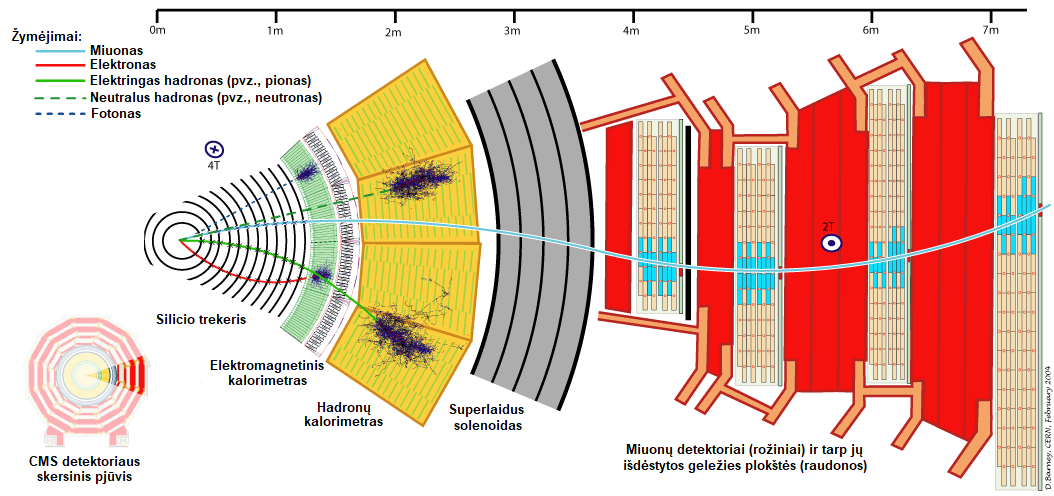
\includegraphics[width=\textwidth]{CMSslice_LT.png}
	\caption{\label{fig:CMSslice}Skersinis CMS detektoriaus pjūvis \cite{CMSslice}.
	Skirtingos linijos žymi įvairių dalelių, išlekiančių iš protonų susidūrimo vietos, trajektorijas.
	Trūki linija žymi elektriškai neutralios dalelės trajektoriją, kuri silicio trekų detektoriuje
	neužfiksuojama.}
\end{figure}

CMS detektoriaus sluoksnius galima pamatyti \ref{fig:CMSslice} paveiksle.
Kiekvienas subdetektorius turi vieną cilindrinę ir dvi antgalių dalis, kurios yra išdėstytos sluoksniais
aplink protonų susidūrimo vietą.
Subdetektorių sluoksniai yra išdėstyti atsižvelgiant į detektuojamų dalelių skvarbą, kiekvienas sluosknis
yra skirtingas ir turi savo paskirtį \cite{CMSexperiment}.

Išsaugoti kiekvieną kas $25$~ns vykstantį įvykį fiziškai yra labai sudėtinga: iš visų detektoriaus elementų
surinkta informacija apie vieną įvykį užima apie $1$ MB \cite{CMScomputing}.
Norint išsaugoti visus įvykius reikėtų ypatingai greitos elektronikos, galinčios išrašyti $~40$~TB duomenų
per sekundę.
Taip pat reikėtų didžiulių duomenų saugojimo pajėgumų, o tai nėra optimalu turint omenyje, jog labai didelė dalis
įvykių tyrėjams nebus įdomi (nepakankamai didelės energijos reakcijos, jau pakankamai ištirti procesai ir pan.).
Taigi, išsaugomų įvykių skaičiui sumažinti naudojama dviejų lygių trigerių sistema \cite{CMStrig}.
Pirmojo lygio trigeris -- tai šalia detektoriaus sumontuota specialiai tam sukurta kompiuterinės
įrangos sistema.
Joje realiu laiku minimaliai apdorojami kalorimetrų bei miuonų detektorių duomenys ir pagal juos per
$4 \; \mathrm{\mu s}$ sistema nusprendžia, ar įvykis turėtų būti išsaugomas tolimesnei analizei. 
Pirmojo lygio trigeris išsaugo maždaug $1$ įvykį iš $10000$.
Aukšto lygio trigeris -- tai superkompiuterių sistema, į kurią atkeliauja pirmojo lygio trigerį
aktyvavę įvykiai.
Čia įvykiai atkuriami pasinaudojant pilna detektoriaus užregistruota informacija, naudojami
griežtesni atrankos kriterijai.
Tai padeda įvykių skaičių sumažinti iki maždaug $1000$ įvykių per sekundę.
Pastarieji yra įrašomi ilgalaikiam saugojimui, kad vėliau galėtų būti analizuojami mokslininkų.

Protonų susidūrimo įvykio vaizdas, pasinaudojant detektoriaus užregistruota informacija, atkuriamas naudojantis
dalelių srauto (angl.\ \textit{Particle Flow}) algoritmu \cite{ParticleFlow}.
Šis algoritmas bando susieti trekų detektoriuje užregistruotus signalus su pataikymais į kalorimetrus arba miuonų
detektorius, taip nustatydamas, kokios dalelės susidarė ir kokie jų parametrai (krūvis, skersinis impulsas,
skersinė energija, pseudosparta ir pan.).
Tokiu būdu gaunamas platus galutinių įvykio produktų sąrašas, leidžiantis pamatyti pilną protonų susidūrimo įvykio vaizdą,
kurį jau gali analizuoti mokslinės tyrimų grupės.

\subsection{Duomenų rinkiniai ir analizės kodai}\label{sec:data}

Šiame darbe buvo naudojami dalinai apdoroti CERN CMS detektoriaus 2016 metais užregistruoti $13$~TeV
energijos protonų susidūrimų duomenys.
Duomenų kiekis atitinka $35.9$~\invfb in-tegruotąjį šviesį, arba $~2 \cdot 10^{15}$ protonų susidūrimų.
Tai yra apie $10$ kartų daugiau įvykių, nei užregistruota $2015$-aisiais metais \cite{DY2019}.

Detektoriaus duomenų interpretavimui buvo pasitelkiami modeliuoto Drell-Yan signalo bei pagrindinių triukšmo
procesų duomenų rinkiniai (signalo ir triukšmo sąvokos aptariamos \ref{sec:sig_bkg}~skyriuje).
Drell-Yan signalo bei $\WJets$ proceso įvykiai buvo sumodeliuoti antros eilės kvantinės chromodinamikos
perturbacijų tikslumu  (angl.\ \textit{next-to-leading order} -- NLO) naudojant \textsc{MadGraph5\_aMC@NLO} įvykių
modeliavimo programą \cite{MG_aMCatNLO}.
Viršūninio kvarko ir antikvarko poros ($t\bar{t}\,$) ir vieno viršūninio kvarko kartu su $W$ bozonu ($tW$ arba
$\tbarW$) įvykiai buvo sumodeliuoti naudojant \textsc{Powheg} \cite{powheg_ttbar, powheg_tW}.
\textsc{Powheg} taip pat įvykius modeliuoja antros eilės QCD perturbacijų tikslumu.
Dviejų bozonų ($WW$, $\WZ$, $\ZZ$) įvykiai buvo sumodeliuoti su \textsc{Pythia8} nulinės eilės perturbacijų tikslumu
(angl.\ \textit{leading order} -- LO) \cite{pythia82}.
Visų modeliuotų įvykių metu vykstantys antriniai procesai, tokie, kaip hadronizacija, spinduliavimas, dalelių skilimai,
pašaliniai protonų susidūrimai ir pan., buvo sumodeliuoti naudojantis \textsc{Pythia8}.
Detektoriaus atsakas į kiekvieną iš sumodeliuotų įvykių buvo modeliuojamas naudojantis \textsc{Geant4} programa
\cite{geant4}.
Eksperimentinių ir modeliuotų duomenų rinkiniai sudaryti vengiant pasikartojimų.

Eksperimente užregistruotų įvykių skaičius yra fiksuotas ir nulemtas skirtingų procesų reakcijų skerspjūvių bei
integruotojo šviesio, kuris priklauso nuo protonų susidūrimų dažnio, protonų pluoštelio matmenų, protonų skaičiaus
viename pluoštelyje, pluoštelių prasikeitimo kampo ir pan.
Tuo tarpu modeliuotų įvykių skaičius gali būti įvairus priklausomai nuo turimų skaičiavimo resursų ir bendru atveju
nesutampa su eksperimente užregistruotu įvykių skaičiumi.
Kad būtų galima palyginti matavimą su modeliavimu, modeliuotų įvykių skaičius turi būti sunormuotas
į išmatuotą integruotąjį šviesį.
Žinant proceso reakcijos skerspjūvį $\sigma$ ir integruotąjį šviesį $\Lumi$, tikėtiniausią įvykių skaičių $N$
gauname iš šių dydžių sandaugos:
\begin{equation}
	N = \sigma\Lumi \; .
\end{equation}
Turimą sumodeliuotų įvykių skaičių sunormuojame į $N$ kiekvienam modeliuotam įvykiui priskirdami normuojantį svorį
$\omega_{i}^{\mathrm{Norm.}}$, kuris apskaičiuojamas taip:
\begin{equation}
	\omega_{i}^{\mathrm{Norm.}} = \omega_{i}^{\mathrm{Gen.}} \frac{ \sigma\Lumi }{ \sum_{i=j}^{N}\omega_{j}^{\mathrm{Gen.}} } \; ,
	\label{eq:NLOweight}
\end{equation}
čia $\omega_{i}^{\mathrm{Gen.}}$ kiekvieno įvykio individualus svoris, priskirtas įvykių modeliavimo programos.
Daugumai procesų $\omega_{i}^{\mathrm{Norm.}}<1$.

Darbe naudoti CMS Drell-Yan tyrimo grupės dalinai atrinkti duomenys yra saugomi Pietų Korėjoje esančiame CMS Tier2
duomenų centre ir užima apie $14$ TB.
Duomenų analizei buvo rašomi C++ programiniai moduliai, kurie buvo leidžiami ROOT aplinkoje \cite{ROOTarticle}.
Duomenų analizė vykdyta dviem etapais: pirmiausia buvo atliekama išmatuotų ir modeliuotų įvykių atranka nuotoliniu
būdu prisijungus prie skaičiavimo centro.
Svarbiausia su atrinktais įvykiais susijusi informacija buvo įrašoma į naujus duomenų failus, kurie užima tik
apie $10$ GB.
Naujai sukurti failai buvo parsisiunčiami į vietinį kompiuterį tolimesnei analizei.
Programinio kodo versijos buvo tvarkomos naudojantis \textit{Github} versijų valdymo sistema.
Visi parašyti analizės kodai yra patalpinti \textit{Github} saugykloje, esančioje adresu
\url{https://github.com/marijusambrozas/DrellYan2016/tree/master/SelectedX}.


\subsection{Signalo ir triukšmo sąvoka}\label{sec:sig_bkg}

Vykdant protonų susidūrimus galutinė įvykio būsena dažnai yra palydima vieno ar kelių kvarkų ir/arba gliuonų
(neskaitant likusių partonų, kurie protonams susiduriant tarpusavyje nesureaguoja ir nulekia apytiksliai tiesiai).
Pavyzdžiui, energingą kvarką arba gliuoną prieš sąveikaudami gali išspinduliuoti reakcijoje dalyvaujantys partonai,
taip pat įvykio metu sukurtos masyvios dalelės (tokios, kaip taonai, $W$, $Z$ ir Higso bozonai) su tam tikra
tikimybe gali skilti į kvarkus ir pan.
Vis dėlto, pavieniai kvarkai arba gliuonai dalelių detektoriais niekada nebūna aptinkami.
Energingi kvarkai arba gliuonai nuolat praranda energiją spinduliuodami papildomus gliuonus, o gliuonai savo ruožtu
dar gali skilti į kvarko-antikvarko poras.
Tokiu būdu lėkdamas vienas partonas sukuria taip vadinamą \ltq{partonų dušą} (angl.\ \textit{parton shower}).
Galiausiai partonų duše esančių dalelių energija pasidaro pakankamai maža, kad perturbatyvusis kvantinės chromodinamikos
aprašymas joms nebetinka -- sąveikos konstanta yra labai didelė, kvarkus atskirti vieną nuo kito reikia begalinės energijos.
Žemose energijose ($<1$~GeV) pasireiškia kvarkų \ltq{įkalinimas} (angl.\ \textit{confinement}): dėl sąveikos stiprumo
kvarkai gali egzistuoti tik grupėmis, kuriose spalvinis krūvis neutralizuojamas.
Taigi, partonų duše esantys kvarkai ir gliuonai pradeda formuoti hadronus (šis procesas vadinamas hadronizacija)
ir vieno energingo partono pėdsaką detektoriuje užfiksuojame kaip kūgio formos dalelių srautą, sudarytą iš daugybės
įvairių rūšių hadronų \cite{Jets}.
Šie hadronų srautai vadinami čiurkšlėmis (angl.\ \textit{jets}).

Vis dėlto, nebūtinai visos čiurkšlėse susidarančios dalelės yra hadronai.
Hadronizacijos proceso metu neretai gali susiformuoti ir fotonai (pavyzdžiui, neutralaus piono skilimo metu).
Taip pat protonų susidūrimo metu vykstant didelės energijos partonų sklaidos procesams galima sukurti sunkiųjų kvarkų,
kurie skyla leptoniškai.
Pavyzdžiui, elektronas arba miuonas gali būti randamas apytiksliai $20\%$ gelminio kvarko sukurtų čiurkšlių
(angl.\ \textit{b-jets}) ir apytiksliai $10\%$ žaviojo kvarko sukurtų čiurkšlių (angl.\ \textit{c-jets}) \cite{LeptonJets}.
Čiurkšlėse susidariusios stipriąja sąveika nesąveikaujančios dalelės neretai pagelbėja mokslininkams nustatant,
kokį kvarką atitinka matoma čiurkšlė \cite{LeptonJets}, tačiau taip pat gali ir suklaidinti -- kartais čiurkšlė gali
būti supainiojama su protonų susidūrimo metu pagamintu leptonu \cite{DY2013, DY7TeVatlas, DY2015, DY8TeVatlas, DY2019, EleID, MuonID}.

Drell-Yan proceso metu susidaro du priešingo elektrinio krūvio izoliuoti leptonai.
Leptono izoliuotumas nustatomas lyginant jo skersinį impulsą su visų kitų artimoje aplinkoje aptiktų dalelių
(patenkančių į $\Delta R = \sqrt{(\Delta\eta)^2 + (\Delta\phi)^2} < 0.3$ formos kūgį, nubrėžtą aplink leptono
trajektoriją, kur $\eta$ -- pseudosparta, $\phi$ -- azimutinis kampas) skersinių impulsų suma:
\begin{equation}
	\label{eq:Iso}
	I^{\mathrm{rel.}}_{\mathrm{PF}} = \frac{1}{p_{\mathrm{T}}} 
	\left[ \sum_{\Delta R<0.3} p_{\mathrm{T}}^{\mathrm{hadron^{\pm}}} +
	\sum_{\Delta R<0.3} p_{\mathrm{T}}^{\mathrm{hadron^0}} + 
	\sum_{\Delta R<0.3} p_{\mathrm{T}}^{\gamma} \right] \; \mathrm{,}
\end{equation}
čia $I^{\mathrm{rel.}}_{\mathrm{PF}}$ -- santykinis leptono izoliuotumas (\ltq{PF} žymi, jog šis dydis apskaičiuojamas
dalelių srauto algoritmo), $\pT$ -- leptono skersinis impulsas,
$p_{\mathrm{T}}^{\mathrm{hadron^{\pm}}}$ -- elektringų hadronų skersiniai impulsai,
$p_{\mathrm{T}}^{\mathrm{hadron^0}}$ -- elektriškai neutralių hadronų skersiniai impulsai,
$p_{\mathrm{T}}^{\gamma}$ -- fotonų skersiniai impulsai \cite{ParticleFlow}.
Sakoma, kad leptonas yra izoliuotas, jeigu pašalinių dalelių skersinių impulsų suma sudaro tik mažą dalį (pvz., $<15\%$)
jo skersinio impulso.

Izoliuotų leptonų pora gali susidaryti ir kitų procesų metu.
Dažni tokio tipo procesai yra šie: viršūninio kvarko ir antikvarko poros ($\ttbar\,$) įvykiai, dviejų masyvių vektorinių bozonų
įvykiai ($WW$, $\WZ$ ir $\ZZ$), vieno viršūninio kvarko ir $W$ bozono įvykiai ($tW$ arba $\tbarW$), o taip pat ir
Drell-Yan proceso taonų kanalas $\DYtau$, kai taonai skyla į elektronus arba miuonus.
Bendru atveju čiurkšlėse susidarę leptonai nėra izoliuoti (jie yra apsupti hadronų srauto).
Vis dėlto, pasitaiko atvejų, kai leptonas yra pakankamai energingas, kad susumuotas aplink lėkusių hadronų ir fotonų
skersinis impulsas sudaro tik mažą dalį leptono impulso.
Labai retais atvejais nutinka ir taip, kai energinga čiurkšlė pralekia hadronų kalorimetrą ir palieka signalą miuonų
detektoriuje.
Jeigu tokio \ltq{netikro} miuono energija yra pakankamai didelė, įmanoma netgi klaidingai pagalvoti, kad jis yra izoliuotas.
Prie šio įvaizdžio gali prisidėti ir neidealus detektoriaus efektyvumas (nebūtinai bus užfiksuotos visos čiurkšlėje
susidariusios dalelės).
Visi įvykiai, kurie analizuojant duomenis atrodo kaip Drell-Yan (signalo) procesas, tačiau tokie nėra, vadinami
\textbf{triukšmo įvykiais}.
Pagrindiniai su klaidingai atpažintomis čiurkšlėmis susiję Drell-Yan proceso triukšmo įvykiai yra $W$ bozono ir  čiurkšlės
įvykiai ($\WJets$) bei stipriosios sąveikos nulemti kelių čiurkšlių įvykiai (sutrumpintai vadinami $\QCD$).
Stengiantis išskirti, kokią dalį detektoriaus registruojamuose pasiskirstymuose sudaro signalo (Drell-Yan),
o kokią -- triukšmo įvykiai, gali būti pasitelkiamas Monte Carlo (MC) modeliavimas ir/arba matavimu grįsti metodai.

\textbf{Monte Carlo modeliavimas} -- tai Monte Carlo metodu sumodeliuoti protonų susidūrimo įvykiai.
Naudoti modeliuoti duomenų rinkiniai yra aprašyti \ref{sec:data}~skyriuje.
Įvykių modeliavimas atliekamas keliais lygmenimis.
Pirmiausia sumodeliuojamas pats protonų susidūrimas ir gaunama, kokios dalelės susidarė jo metu.
Tada modeliuojami po susidūrimo vykstantys antriniai procesai, tokie, kaip hadronizacija, spinduliavimas, dalelių skilimai,
pašaliniai mažos energijos protonų susidūrimai, vykstantys tuo pačiu metu (angl.\ \textit{pile-up}).
Galiausiai modeliuojama, kaip įvykio produktai sąveikauja su medžiaga -- detektoriaus komponentais.
Tokį virtualų eksperimentą kartojant daug kartų galima gauti vidutinį rezultatą, kuris yra palyginamas su realiu eksperimentu.
Vis dėlto, sumodeliuoti įvykius taip, kad virtualaus eksperimento sąlygos idealiai atitiktų realaus eksperimento sąlygas,
yra praktiškai neįmanoma.
Atsižvelgiant į kai kuriuos neatitikimus modeliuotiems įvykiams gali būti pritaikomos CMS eksperimento mokslinių grupių
rekomenduojamos pataisos.
Tačiau vis tiek egzistuoja modeliavimo neapibrėžtumų, kurie kenkia įverčio kokybei (pavyzdžiui, nepakankamos žinios apie
atskirų triukšmo procesų įvykių tikėtinumus, neidealus detektoriaus atsako modeliavimas, papildomi protonų susidūrimai ir pan.).
Šios problemos gali būti sušvelnintos triukšmo įvykių skaičiaus įvertinimui naudojant matavimu grįstus metodus.

\textbf{Matavimu grįsti metodai} apjungia matavimą ir modeliavimą, kad būtų gautas kuo tikroviškesnis įvykių skaičiaus įvertis.
Matavimu grįstų metodų veikimo principas remiasi signalo ir kontrolinės sričių apibrėžimais.
Signalo sritis pasirenkama taip, kad į ją patektų kuo daugiau signalo ir kuo mažiau triukšmo įvykių.
Kontrolinė sritis pasirenkama taip, kad į ją patektų kuo daugiau triukšmo ir kuo mažiau signalo įvykių.
Sritys apibrėžiamos tam tikrais užregistruotus įvykius apibūdinančių parametrų apribojimais.
Šie parametrai gali būti įvairūs: tam tikrų dalelių ar čiurkšlių skaičius, trajektorijų izoliuotumas ir pan.
Signalo ir kontrolinė sritys turi būti nepersiklojančios.
Matavimu grįsti metodai triukšmo įvykių skaičių, apskaičiuotą kontrolinėje srityje, transformuoja į triukšmo įvykių skaičių,
esantį signalo srityje.
Jei triukšmo įvykyje susidaro dvi nestabilios dalelės, kurios skyla į izoliuotus leptonus nepriklausomai,
jo indėlis gali būti įvertintas $\emu$ metodu.
Taip pat eksperimentinėje didelių energijų fizikoje ganėtinai populiarūs yra fizikinio objekto klaidingo atpažinimo ir ABCD metodai.
Jie naudojami įvertinti skaičiui tokių triukšmo įvykių, kurių metu susidaro viena ar kelios čiurkšlės.
Anksčiau atliktame darbe Drell-Yan proceso triukšmo įvykių skaičiui įvertinti buvo taikomas $\emu$ metodas, o šiame darbe gilinamasi
į klaidingo atpažinimo metodą.

\subsection{Klaidingo atpažinimo metodas}
Fizikinio objekto klaidingo atpažinimo metodas buvo naudojamas įvertinti $\WJets$ ir $\QCD$ įvykių skaičiui.
Tai yra tokie triukšmo įvykiai, kuriuose viena arba dvi čiurkšlės buvo atpažintos, kaip miuonai.
Klaidingo atpažinimo metodas remiasi tikimybės, kad klaidingai atpažintas fizikinis objektas pateks į signalo sritį
(angliškai ši tikimybė vadinama \textit{fake rate}), įvertinimu.

Kontrolinė sritis buvo apibrėžta invertuojant miuono izoliuotumo kriterijų -- reikalaujama, kad miuono kandidato
trajektorija būtų neizoliuota nuo kitų dalelių trajektorijų (tai neretai yra čiurkšlės arba miuono, susidariusio čiurkšlėje, požymis).
Tada klaidingo atpažinimo tikimybe vadiname dydį, nusakantį, kokia dalis visų miuonais atpažintų čiurkšlių turi galimybę patekti
į signalo sritį:
\begin{equation} \label{eq:FR}
	f_{\mathrm{signal} \,| \,\mathrm{Jet}} =
	\frac{N^{\QCD}_{\mathrm{signal}}}{N^{\QCD}_{\mathrm{signal}}+N^{\QCD}_{\mathrm{control}}} \; ,
\end{equation}
čia $f_{\mathrm{signal} \,| \,\mathrm{Jet}}$ -- klaidingo atpažinimo tikimybė, $N^{\QCD}_{\mathrm{signal}}$ -- į signalo sritį
patenkančių miuonais atpažintų čiurkšlių skaičius, $N^{\QCD}_{\mathrm{control}}$ -- į kontrolinę sritį patenkančių kaip miuonai
atpažintų čiurkšlių skaičius.
Indeksas $\QCD$ žymi faktą, kad klaidingo atpažinimo tikimybės įvertinimui turėtume naudoti tik $\QCD$ įvykius, t.y., tuos
įvykius, kuriuose susidaro vien tik čiurkšlės, todėl bet koks tokiuose įvykiuose atpažintas miuonas yra kilęs iš čiurkšlės.
Vis dėlto, į kontrolinę sritį gali patekti ne vien $\QCD$, bet ir tokie įvykiai, kuriuose yra tikrų, tik dėl įvairių
priežasčių neizoliuotų miuonų.
Pavyzdžiui, dėl mažo miuono impulso laboratorinėje atskaitos sistemoje jis gali neišsiskirti.

Norint teisingai įvertinti klaidingo atpažinimo tikimybę, iš eksperimento metu užregistruotų duomenų reikėjo išskirti $\QCD$
proceso įvykius.
$\QCD$ įvykių išskyrimui buvo pasitelkti modeliuoti duomenų rinkiniai.
Paprasčiausias variantas išskirti $\QCD$ įvykius būtų iš atranką praėjusių eksperimento metu užregistruotų įvykių skaičiaus
atimti modeliuotą visų su $\QCD$ nesusijusių procesų įvykių skaičių:
\begin{equation}
	\begin{gathered}
		N^{\QCD}_{i} = N^{\mathrm{Data}}_{i} - \left( N^{\mathrm{DY}}_{i} +
		N^{\WJets}_{i} + N^{\ttbar}_{i} + N^{tW+\tbarW}_{i} +
		N^{WW+\WZ+\ZZ}_{i} \right)^{\mathrm{MC}}; \\
		\hspace{280pt} i = \mathrm{signal}, \, \mathrm{control},
	\end{gathered}
\end{equation}
tačiau šis metodas nėra tinkamas, nes pašalinių įvykių skaičius yra pakankamai didelis, o taip pat įvykiai, kuriuose leptonai
nėra izoliuoti, yra prasčiau sumodeliuoti ir ne taip gerai sutampa su matavimu.
Tikslesniam $\QCD$ įvykių skaičiaus įvertinimui buvo naudojami du skirtingi metodai:
\begin{enumerate}
	\item Santykio metodas -- $\QCD$ įvykių skaičius įvertinamas iš matavimo paėmus procentinę $\QCD$ įvykių dalį, kuri buvo apskaičiuota
	pasinaudojant modeliavimu:
	\begin{equation}
		\begin{gathered}
			N^{\QCD}_{i} = N^{\mathrm{Data}}_{i} \cdot \left(\frac{N^{\QCD}_{i}}
			{N^{\QCD}_{i} + N^{\mathrm{DY}}_{i} + N^{\WJets}_{i} +
			N^{\ttbar}_{i} + N^{tW+\tbarW}_{i} + N^{WW+\WZ+ZZ}_{i}} \right)^{\mathrm{MC}}; \\
			\hspace{300pt} i = \mathrm{signal}, \, \mathrm{control}.
		\end{gathered}
	\end{equation}
	\item Šablonų pritaikymo (angl.\ \textit{template fitting}) metodas -- $\QCD$ įvykių skaičius įvertinamas prie tam tikro
	išmatuoto pasiskirstymo pritaikius skirtingų procesų pasiskirstymų šablonus, darant prielaidą, kad įvykių tikimybinis
	pasiskirstymas yra teisingas, o normavimo amplitudė netiksli.
	Skirtingų procesų šablonai dažniausiai (ir šiame darbe) gaunami iš modeliavimo.
	Pasiskirstymas, kurio šablonai pritaikomi prie matavimo, turi būti pasirenkamas toks, kuris leistų pakankamai gerai
	atskirti $\QCD$ nuo kitų procesų (pasiskirstymų forma turėtų būti skirtinga).
	Šiuo atveju buvo naudojami miuono trajektorijos izoliuotumo pasiskirstymo šablonai.
	Turint detektoriaus išmatuotą pasiskirstymą ir skirtingų procesų šablonus, stengiamasi gauti geriausią sutapimą tarp matavimo ir
	šablonų sumos varijuojant kiekvienam šablonui priskirtus svorinius daugiklius:
	\begin{equation}
		\begin{gathered}
			N^{\mathrm{Data}}_{i}(I^{\mathrm{rel.}}_{\mathrm{PF}}) \approx
			\lambda^{\mathrm{fit}}_{\,i}\, N^{\,\QCD}_{i}(I^{\mathrm{rel.}}_{\mathrm{PF}}) +
			\epsilon^{\,\mathrm{fit}}_{\,i}\, N^{\,\mathrm{DY}}_{i}(I^{\mathrm{rel.}}_{\mathrm{PF}}) +
			\zeta^{\,\mathrm{fit}}_{\,i}\, N^{\,\WJets}_{i}(I^{\mathrm{rel.}}_{\mathrm{PF}}) + \\[7pt] +
			\theta^{\,\mathrm{fit}}_{i}\, N^{\,\ttbar}_{i}(I^{\mathrm{rel.}}_{\mathrm{PF}}) +
			\kappa^{\,\mathrm{fit}}_{\,i}\, N^{\,tW}_{i}(I^{\mathrm{rel.}}_{\mathrm{PF}}) + 
			\xi^{\,\mathrm{fit}}_{i}\, N^{\,\tbarW}_{i}(I^{\mathrm{rel.}}_{\mathrm{PF}}) +
			\tau^{\,\mathrm{fit}}_{i}\, N^{\,WW}_{i}(I^{\mathrm{rel.}}_{\mathrm{PF}}) + \\[7pt] +
			\chi^{\,\mathrm{fit}}_{\,i}\, N^{\,\WZ}_{i}(I^{\mathrm{rel.}}_{\mathrm{PF}}) +
			\psi^{\,\mathrm{fit}}_{i}\, N^{\,\ZZ}_{i}(I^{\mathrm{rel.}}_{\mathrm{PF}});
			\hspace{74pt} i = \mathrm{signal}, \, \mathrm{control}.
		\end{gathered}
	\end{equation}
	Čia $\lambda^{\mathrm{fit}}_{\,i}$, $\epsilon^{\,\mathrm{fit}}_{\,i}$ ir t.t.\ -- varijuojami daugikliai,
	kuriuos keičiant bandoma gauti geriausią šablonų sumos sutapimą su matavimu mažiausių kvadratų metodu.
	Idealiu atveju šie daugikliai turėtų būti lygūs vienetui. 
	Gavus daugiklių vertes klaidingo atpažinimo tikimybė įvertinama naudojant modeliuotą $\QCD$ įvykių skaičių, padaugintą
	iš gautojo daugiklio vertės:
	\begin{equation}
		f_{\mathrm{signal} \,| \,\mathrm{Jet}} =
		\frac{\lambda^{\mathrm{fit}}_{\,\mathrm{signal}}\, N^{\,\QCD \; \mathrm{MC}}_{\mathrm{signal}}}
		{\lambda^{\mathrm{fit}}_{\,\mathrm{signal}}\, N^{\,\QCD \; \mathrm{MC}}_{\mathrm{signal}} +
		\lambda^{\mathrm{fit}}_{\,\mathrm{control}}\, N^{\,\QCD \; \mathrm{MC}}_{\mathrm{control}}}\, .
	\end{equation}
	Svarbu atkreipti dėmesį, kad, nors šablonų pritaikymas daromas izoliuotumo pasiskirstymui, šis pasiskirstymas klaidingo
	atpažinimo tikimybėje neatsispindi: įvertindami klaidingo atpažinimo tikimybę naudojame tik gautą svorinio daugiklio vertę.
	Šablonų pritaikymo metodas yra laikomas tikslesniu nei santykio metodas, todėl jis buvo naudojamas kaip pagrindinis rezultatas.
\end{enumerate}

Apskaičiavus klaidingo atpažinimo tikimybę buvo galima ją pritaikyti įvertinant, koks kiekis klaidingai atpažintų čiurkšlių
galėjo patekti į signalo sritį.
Drell-Yan proceso atveju, kai ieškoma dviejų leptonų, galimas dvejopas klaidingo atpažinimo nulemtas triukšmas: $\WJets$ atveju
klaidingai atpažįstamas tik vienas leptonas, o $\QCD$ atveju -- abu.
Pilnas į signalo sritį patenkančių įvykių skaičius gali būti išreikštas taip:
\begin{multline}
	\label{eq:realfake}
	N_{\mathrm{signal, \; signal}} = N_{l, \, l} \cdot f^2_{\mathrm{signal} \,| \, l} +
	N_{l, \, \mathrm{Jet}} \cdot f_{\mathrm{signal} \,| \, l} \cdot f_{\mathrm{signal} \,| \,\mathrm{Jet}} +
	N_{\mathrm{Jet, \, Jet}} \cdot f^2_{\mathrm{signal} \,| \,\mathrm{Jet}} \, ,
\end{multline}
čia $l$ žymi tikrą leptoną, $N_{l, \, l}$, $N_{l, \, \mathrm{Jet}}$, $N_{\mathrm{Jet, \, Jet}}$ -- įvykių,
kurių metu susidarė atitinkamai du leptonai, leptonas ir čiurkšlė, arba dvi čiurkšlės, skaičius,
$f_{\mathrm{signal} \,| \,\mathrm{Jet}}$ -- klaidingo atpažinimo tikimybė, $f_{\mathrm{signal} \,| \,l}$ -- tikimybė,
kad tikras leptonas bus atpažintas teisingai (dar vadinama efektyvumu).

Ši formulė yra supaprastinta: iš tikrųjų klaidingo atpažinimo tikimybė buvo įvertinta kaip funkcija nuo miuono kandidato
skersinio impulso ir pseudospartos, todėl kiekvienai dalelei $f_{\mathrm{signal} \,| \,\mathrm{Jet}}$  gali būti skirtingas dydis.
Verta atkreipti dėmesį į tai, jog \eqref{eq:realfake} lygybės dešinė pusė susideda iš trijų dėmenų.
Pirmasis dėmuo yra siejamas su tikrų leptonų įvykiais: Drell-Yan signalu ir triukšmo procesais, kurių metu susidaro tikri leptonai.
Antrasis dėmuo yra siejamas su vieno tikro leptono ir vienos klaidingai atpažintos čiurkšlės įvykiais
(dominuojantis procesas -- $\WJets$), o trečiasis -- su dviejų klaidingai atpažintų čiurkšlių įvykiais -- $\QCD$ triukšmu.
Pritaikę klaidingo atpažinimo tikimybę galime įvertinti \eqref{eq:realfake} išraiškos dešinėje pusėje esančius antrąjį ir trečiąjį dėmenis.
Antrajame dėmenyje esantis $N_{l, \, \mathrm{Jet}}$ gali būti įvertintas pasinaudojus įvykiais, kuriuose susidarė vienas tikras
leptonas, patenkantis į signalo sritį, ir viena klaidingai atpažinta čiurkšlė, patenkanti į kontrolinę sritį:
\begin{equation}
	\label{eq:FRWjets}
	N_{l, \, \mathrm{Jet}} = \frac{N^{\WJets}_{\mathrm{signal, \, control}}}
	{f_{\mathrm{signal} \,| \, l}\cdot f_{\mathrm{control} \,| \, \mathrm{Jet}}} =
	\frac{N^{\WJets}_{\mathrm{signal, \, control}}}
	{f_{\mathrm{signal} \,| \, l}\cdot \left( 1 - f_{\mathrm{signal} \,| \, \mathrm{Jet}} \right)}	\, ,
\end{equation}
čia $N^{\WJets}_{\mathrm{signal, \, control}}$ -- $\WJets$ įvykių skaičius, kurių metu susidariusi čiurkšlė
klaidingai atpažįstama, bet patenka į kontrolinę sritį.
Trečiajame \eqref{eq:realfake} išraiškos dėmenyje esantis $N_{\mathrm{Jet, \, Jet}}$ gali būti įvertintas pasinaudojus įvykiais,
kuriuose dvi klaidingai atpažintos čiurkšlės patenka į kontrolinę sritį:
\begin{equation}
	\label{eq:FRQCD}
	N_{\mathrm{Jet, \, Jet}} = \frac{N^{\QCD}_{\mathrm{control, \, control}}}{f^2_{\mathrm{control} \,| \,\mathrm{Jet}}} =
	\frac{N^{\QCD}_{\mathrm{control, \, control}}}{\left(1-f_{\mathrm{signal} \,| \,\mathrm{Jet}}\right)^2} \, ,
\end{equation}
čia $N^{\QCD}_{\mathrm{control, \, control}}$ -- $\QCD$ įvykių skaičius, kuriuose dvi klaidingai atpažintos čiurkšlės patenka į
kontrolinę sritį.
Įstatę \eqref{eq:FRWjets} ir \eqref{eq:FRQCD} išraiškas į \eqref{eq:realfake}, gauname:
\begin{equation}
	\label{eq:FRapply}
	N_{\mathrm{signal, \; signal}} = N_{l, \, l} \cdot f^2_{\mathrm{signal} \,| \,l} +
	N^{\WJets}_{\mathrm{signal, \, control}} \cdot
	\frac{f_{\mathrm{signal} \,| \, \mathrm{Jet}}} {1 - f_{\mathrm{signal} \,| \, \mathrm{Jet}}} + 
	N^{\QCD}_{\mathrm{control, \, control}} \cdot
	\frac{f^2_{\mathrm{signal} \,| \,\mathrm{Jet}}}
	{\left(1-f_{\mathrm{signal} \,| \,\mathrm{Jet}} \right)^2}\, .
\end{equation}
Taigi, įvertinus klaidingo atpažinimo tikimybę $f_{\mathrm{signal} \,| \,\mathrm{Jet}}$, $\QCD$ ir $\WJets$ triukšmo įvykių
skaičių galima įvertinti apskaičiuojant šių įvykių skaičių kontrolinėje srityje ir perkeliant gautą rezultatą į
signalo sritį panaudojant po vieną daugiklį
$f_{\mathrm{signal} \,| \,\mathrm{Jet}}/(1-f_{\mathrm{signal} \,| \,\mathrm{Jet}})$  kiekvienam miuonui.
Čia taip pat naudojamos supaprastintos išraiškos ir realiai klaidingo atpažinimo tikimybė kiekvienai dalelei gali būti skirtinga.

Kaip ir įvertinant klaidingo atpažinimo tikimybę, į kontrolinę sritį gali patekti ir su $\WJets$ ar $\QCD$ nesusiję įvykiai.
Šiuos įvykius reikia atmesti.
Jeigu pašalinių įvykių yra mažai, jų indėlį galima atmesti iš eksperimento metu išmatuoto rezultato atimant modeliuotus
pasiskirstymus.
Priešingu atveju reikia naudotis kokia nors kita technika.
Šiame darbe dydis $N^{\WJets}_{\mathrm{signal, \, control}}$ buvo įvertintas naudojantis šablonų pritaikymu (žr.\ \ref{sec:FRresults} skyrių).


\subsection{Matavimo paklaidų įvertinimas}\label{sec:uncertainties}

Analizuojant protonų susidūrimus laikoma, kad įvykių skaičius yra pasiskirstęs pagal Puasono dėsnį.
Puasono pasiskirstymu aprašomo įvykių skaičiaus standartinis nuokrypis yra lygus kvadratinei šakniai iš labiausiai
tikėtino įvykių skaičiaus.
Atliekant realų eksperimentą, labiausiai tikėtinas įvykių skaičius nėra tiksliai žinomas, todėl atranką praėjusių
įvykių skaičiaus statistinio neapibrėžtumo verte laikoma kvadratinė šaknis iš užregistruoto įvykių skaičiaus.

Kai modeliuoti įvykiai turi nelygius vienetui svorius, jų skaičiaus $N$ statistinis neapibrėžtumas $(\Delta N)_{\mathrm{Stat.\,}}$
įvertinamas kaip kvadratinė šaknis iš modeliuotų įvykių svorių kvadratų sumos:
\begin{equation}
	(\Delta N)_{\mathrm{Stat.\,}} = \sqrt{\sum_{i=1}^{N}w_{i}^{2}} \; ,
	\label{eq:Sumw2Unc}
\end{equation}
čia $$w_{i}=w_{i}^{\mathrm{Norm.}} \cdot \prod_{p=1}^{N_{\mathrm{Pat.}}}w_{i}^{p} \; ,$$
kur $w_{i}^{\mathrm{Norm.}}$ -- modeliuoto įvykio normuojantis svoris, gaunamas iš \eqref{eq:NLOweight} išraiškos,
$w_{i}^{p}$ -- modeliuotam įvykiui pataisos $p$ priskirtas svorinis daugiklis, $N_{\mathrm{Pat.}}$ -- pritaikytų
skirtingų pataisų skaičius.
Modeliuotiems įvykiams taikytos pataisos yra aprašytos \ref{sec:corrections}~skyriuje.
Jeigu modeliuotų įvykių turime daugiau, nei buvo užregistruota eksperimento metu, jiems bus priskiriami mažesni už
vienetą svoriai ir sunormuoto įvykių skaičiaus statistinė paklaida bus mažesnė nei eksperimento metu užregistruotų
įvykių.
Tai yra vienas iš modeliavimo privalumų, kai modeliuojami mažo tikėtinumo įvykiai.
Tuo tarpu, kai modeliuojami labai didelio tikėtinumo įvykiai, priklausomai nuo sumodeliuoto įvykių skaičiaus
jiems gali būti priskiriami labai dideli svoriai.
Tokiu atveju statistinis įvykių skaičiaus neapibrėžtumas bus gerokai didesnis nei detektoriaus užregistruotiems įvykiams.
Tai yra vienas iš modeliavimo trūkumų ir viena iš pagrindinių priežasčių, kodėl naudojamas klaidingo atpažinimo metodas
$\QCD$ ir $\WJets$ įvykių skaičiaus įvertinimui -- jų reakcijos skerspjūviai yra labai dideli ir norint juos kokybiškai
sumodeliuoti reikia ypatingai didelių skaičiavimo resursų.
Jeigu įvykiams priskiriami vienetiniai svoriai, iš \eqref{eq:Sumw2Unc} išraiškos gauname, kad įvykių
skaičiaus paklaida lygi kvadratinei šakniai iš įvykių skaičiaus, taigi, ši formulė tinkama ir eksperimento
metu užregistruotų įvykių skaičiaus statistinio neapibrėžtumo įvertinimui.
Fizikinio objekto klaidingo atpažinimo metodu įvertinto triukšmo įvykių skaičiaus statistinis neapibrėžtumas taip
pat buvo įvertintas paimant kvadratinę šaknį iš gauto rezultato, nes klaidingo atpažinimo tikimybė yra naudojama
kaip svorinis daugiklis, kuris bendru atveju yra labai mažas, todėl neapibrėžtumas, įvertintas naudojantis
\ref{eq:Sumw2Unc} formule būtų netikroviškai mažas.

Galimiems sisteminiams nukrypimams įvertinti CMS statistikos komitetas rekomenduoja turėti bent du skirtingais būdais
atliktus matavimus, kurie, idealiu atveju, turėtų duoti sutampančius įverčius.
Kadangi tikroji vertė, kurią bandoma išmatuoti, yra nežinoma, daroma prielaida, jog skirtingi įverčiai yra
lygiaverčiai ir nepriklausomi, o tikroji vertė yra artimoje aplinkoje.
Tokiu atveju skirtumo tarp dviejų skirtingų rezultatų absoliučioji vertė yra pakankamai saugus sisteminės matavimo
paklaidos įvertis.

Šiame darbe buvo matuojamas Drell-Yan proceso triukšmo įvykių skaičius, o turimi du skirtingi įverčiai buvo gauti naudojant
skirtingas klaidingo atpažinimo tikimybės įvertinimo metodikas: santykio ir šablonų pritaikymo metodą.
Taigi, pagrindinė $\QCD$ ir $\WJets$ įvykių skaičiaus įverčio sisteminės paklaidos sudedamoji dalis buvo įvertinta pagal
tokią formulę:
\begin{equation}
	(\Delta N_{ll}^{\mathcal{P} \; \mathrm{įvert.}})_{\mathrm{Sist.\,}} =
	\left| N_{ll}^{\mathcal{P} \; \mathrm{įvert.}}(\mathrm{šabl.}) -
	N_{ll}^{\mathcal{P} \; \mathrm{įvert.}}(\mathrm{sant.}) \right| \;  ;
	\;\;\;\;\; \mathcal{P} = \QCD, \; \WJets \; ,
	\label{eq:systUncFR}
\end{equation}
čia \ltq{įvert.}\ žymi matavimu grįstą įvertį, \ltq{fit.}\ žymi klaidingo atpažinimo tikimybei įvertinti naudotą šablonų
pritaikymo metodą, o \ltq{sant.}\ -- santykio metodą.

Kadangi klaidingo atpažinimo tikimybei įvertinti buvo naudojamas baigtinis įvykių skaičius, ji turi savo statistinį neapibrėžtumą,
kuris neatsispindi galutinio triukšmo įvykių skaičiaus įverčio statistiniame neapibrėžtume.
Dėl šios priežasties klaidingo atpažinimo tikimybės statistinis neapibrėžtumas buvo įskaitomas laikant jį papildomu indėliu į
sisteminę įverčio paklaidą.
Skirtingos paklaidos dedamosios, laikant, kad jos yra tarpusavyje nepriklausomos, buvo sudedamos pagal Pitagoro teoremą.

\section{Rezultatai ir jų aptarimas}

\subsection{Įvykių atranka}\label{sec:selection}
Ne visi detektoriumi užregistruoti duomenys yra tinkami fizikinei analizei.
Norint iš $2016$-aisiais metais CMS detektoriaus užregistruotų protonų priešpriešinių susidūrimų duomenų išskirti svarbią
ir kokybišką informaciją buvo vykdoma įvykių atranka pagal kriterijus, kurie turėtų atmesti kiek įmanoma daugiau triukšmo
įvykių ir tuo pačiu išsaugoti kuo daugiau signalo įvykių.
Taip pat buvo apribojama tyrimo fazinė erdvė, paliekant tik tas sritis, kuriose detektoriaus veikimas yra efektyviausias.
Visi taikyti atrankos kriterijai yra pateikti \ref{table:selection}~lentelėje.

\begin{table}[b!]
	\begin{tabular}{|c|c|}
		\hline
		\textbf{Kriterijaus tipas} & \textbf{Reikalavimas} \\
		\hline\hline
		\multirow{3}{12em}{\centering Aukšto lygio trigeris} & \ttt{HLT\_IsoMu24} arba \ttt{HLT\_IsoTkMu24} \\ \cline{2-2}
			& \multirow{2}{17em}{\centering Bent vienas miuonas turi būti aktyvavęs trigerį} \\
		 & \\
		\hline\hline
		\multirow{2}{12em}{\centering Kinematiniai reikalavimai} & $p_{\mathrm{T \, 1}} > 28$~GeV, $p_{\mathrm{T \, 2}} > 17$~GeV \\ \cline{2-2}
		 & $|\eta_1| < 2.4$, $|\eta_2| < 2.4$ \\
		\hline\hline
		\multirow{2}{12em}{\centering Dalelės identifikavimo reikalavimai} & \ttt{TightID} reikalavimai \\ \cline{2-2}
		 & $I_{\mathrm{PF}}^{\mathrm{rel.}}<0.15$ \\
		\hline\hline
		\multirow{5}{12em}{\centering Reikalavimai geresniam signalo išskyrimui} &
			\multirow{3}{17em}{\centering Pasirenkami 2 miuonai, kuriuos galima tiksliausiai suvesti į vieną pirminę viršūnę su $\chi^2<20$} \\
		 & \\
		 & \\ \cline{2-2}
		 & Priešingi elektriniai krūviai \\ \cline{2-2}
		 & Plokštuminis kampas $< \pi - 0.005$~rad \\
		\hline
	\end{tabular}
	\caption{\label{table:selection}Apibendrinti įvykių atrankos kriterijai. Indeksai $1$ ir $2$ žymi atitinkamai greitesnįjį
	ir lėtesnįjį miuoną.}
\end{table}

Atrenkant įvykius buvo naudojamas aukšto lygio vieno miuono trigeris, kuris aktyvuojamas aptikus bent vieną
miuoną su skersiniu impulsu, didesniu nei $24$~GeV.
Miuonas turi būti atpažintas pasinaudojant trekų detektoriaus ir miuonų detektorių informacija.
Kiekvienam miuonui iš trigerį aktyvavusių įvykių buvo taikomi \ttt{TightID} reikalavimai \cite{MuonID}, skirti sumažinti atranką
praeinančių netikrų miuonų, bei miuonų, atsiradusių iš antrinių procesų, skaičių.
\ttt{TightID} reikalavimus atitinka virš $95\%$ protonų susidūrimų metu sukurtų tikrų ir mažiau nei $0.3\%$ netikrų
miuonų \cite{MuonID}.
Taip pat kiekvienam miuonui buvo taikomas trajektorijos izoliuotumo reikalavimas: pašalinių dalelių, aptiktų
$\Delta R < 0.3$ pločio kūgyje, nubrėžtame aplink miuono trajektoriją, skersinių impulsų suma negali
viršyti $15\%$ miuono skersinio impulso vertės.
Įvykiai, kuriuose nėra bent dviejų miuonų, atitinkančių išvardintus kriterijus buvo iškart atmetami.
Likusiems įvykiams buvo taikomas reikalavimas, kad miuonų poros trajektorijas būtų galima pakankamai tiksliai
suvesti į vieną pirminę
viršūnę, taip pat buvo reikalaujama bei kad suporuoti miuonai būtų priešingų elektrinių krūvių.
Įvykyje esant kelioms reikalavimus atitinkančioms poroms iš jų buvo išrenkama ta, kurią eina tiksliausiai suvesti į bendrą viršūnę.
Tam, kad būtų išvengta kosminės spinduliuotės miuonų aptikimo, buvo taikomas papildomas kriterijus, reikalaujantis,
kad plokštuminis kampas tarp dviejų miuonų trajektorijų būtų mažesnis, nei $\pi-0.005$~rad.

Atranką praėjo iš viso apie $2.3\cdot10^7$ eksperimento metu užregistruotų įvykių.
Pagrindinis matuojamas dydis buvo atranką praėjusių miuonų porų invariantinė masė.
Iš jų verčių buvo brėžiama invariantinės masės histograma, apimanti masės sritį nuo $15$ iki $3000$~GeV.

\subsection{Pataisos}\label{sec:corrections}
Šiame skyriuje aprašomos pataisos buvo pritaikytos ankstesniame darbe \cite{MAk2}, tačiau jų rezultatai yra
esminiai ir šiam darbui, nes jame naudojami tie patys duomenų rinkiniai.
Todėl pagrindiniai pataisų pritaikymo žingsniai su jų pagrindimu yra pateikiami ir šiame darbe.
Kai kurie grafikai buvo atnaujinti ištaisius kode buvusias klaidas.

Įprastai per vieną protonų pluoštelių prasikeitimą (angl.\ \textit{bunch crossing}) vidutiniškai susiduria
apie 23 protonų poros \cite{CMSLumi}.
Tuo pačiu metu vykstantys pašaliniai protonų susidūrimai turi įtakos užregistruoto įvykio atkūrimo kokybei.
Šį efektą bandoma simuliuoti modeliuotuose įvykiuose, tačiau dažniausiai tikimybinis protonų susidūrimų
skaičiaus (per vieną prasikeitimą) pasiskirstymas matavime ir modeliavime nesutampa.
Nesutapimą iš dalies nulemia atsitiktinės susidūrimų fliuktuacijos.
Nemažą įtaką tam turi ir Didžiojo hadronų greitintuvo technikų tyrinėjimai keičiant protonų spindulio intensyvumą,
pluoštelių skaičių, jų persiklojimo tūrį ir pan.
Nesutapimą tarp išmatuoto ir modeliuoto protonų susidūrimų tankio bandoma sumažinti taikant protonų susidūrimo
skaičiaus pataisas -- kiekvienam modeliuotam įvykiui priskiriamas papildomas svoris pagal tai, koks protonų
susidūrimų skaičius jame buvo sumodeliuotas.
Pataisa buvo taikoma darant prielaidą, kad protonų susidūrimo skerspjūvis greitintuve yra lygus $64$~mb
($6.4 \cdot 10^{-30} \, \mathrm{m}^2)$.
Išmatuoti ir modeliuoti atkurtų pirminių viršūnių skaičiaus pasiskirstymai atranką praėjusiuose įvykiuose
prieš ir po pataisos pateikiami \ref{fig:PUba}~pav.
Čia ir toliau paveikslų apatinėse dalyse pateikiami eksperimentinio ir modeliuoto rezultatų santykio grafikai.
Pritaikius pataisą $10$-$30$ pirminių viršūnių skaičiaus srityje, į kurią patenka apie $91\%$ visų įvykių,
eksperimentinis ir modeliuotas pasiskirstymai pradėjo sutapti labai gerai -- skirtumas neviršija $9\%$.

Miuonų poros invariantinės masės matavimo kokybei ženklios įtakos turi miuonų skersinio impulso matavimo tikslumas.
Dėl šios priežasties visiems užregistruotiems miuonams buvo pritaikytos Ročesterio mokslinės grupės pateikiamos
miuonų impulso matavimo skalės pataisos \cite{RocCorr}.

Dėl modeliavimo netobulumo dažnai nesutampa tam tikros realaus ir virtualaus eksperimento sąlygos.
Kiekvienam miuonų poros įvykiui buvo priskiriami svoriniai daugikliai, priartinantys modeliuotus trigerio
suveikimo bei miuono trajektorijos atkūrimo, atpažinimo ir izoliuotumo įvertinimo efektyvumus prie išmatuotųjų verčių.
Kiekvieno suvidurkinto daugiklio vertė buvo nustatoma pagal leptono skersinio impulso ir pseudospartos vertes.
Tipinė svorinio daugiklio vertė yra apie $0.9$.
Invariantinės masės pasiskirstymai prieš ir po šių pataisų pritaikymo pateikiami atitinkamai \ref{fig:invMba}~pav.
Pritaikius minėtas pataisas sutapimas tarp eksperimento ir modeliavimo pagerėjo vidutiniškai apie $10\%$.

Yra pastebėta, kad pirmos eilės perturbacijų tikslumu modeliuojant viršūninių kvarkų poros ($\ttbar\,$)
įvykius, gaunami skersinių impulsų pasiskirstymai turi nesutapimų su nustatytaisiais eksperimentiškai \cite{ttbarPT}.
Juos buvo bandoma ištaisyti modeliuotiems viršūninių kvarkų poros įvykiams priskiriant viršūninio kvarko tyrimo grupės
siūlomus svorius, kurie skirti priartinti modeliuotą skersinių impulsų pasiskirstymą prie naujausių eksperimentinių rezultatų.
Svorių vertės nustatomos pagal kvarkų skersinių impulsų $p_{t \; \mathrm{T}}$ vertes.
Tipinės svorių vertės yra didesnės už $1$, kai abiejų kvarkų $p_{t \; \mathrm{T}}<120 \, \mathrm{GeV}$, ir mažesnės už $1$,
kai $p_{t \; \mathrm{T}}>120 \, \mathrm{GeV}$.

\begin{figure}[b!]
	\RawFloats
	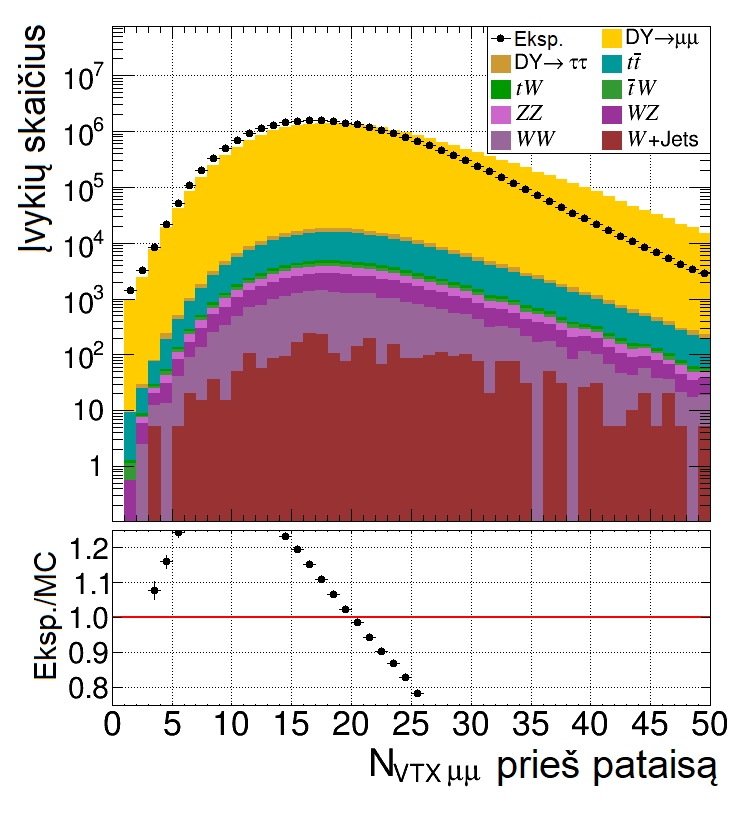
\includegraphics[width=0.48\textwidth]{Kursinis3/mumu_nVTX_before.png}
	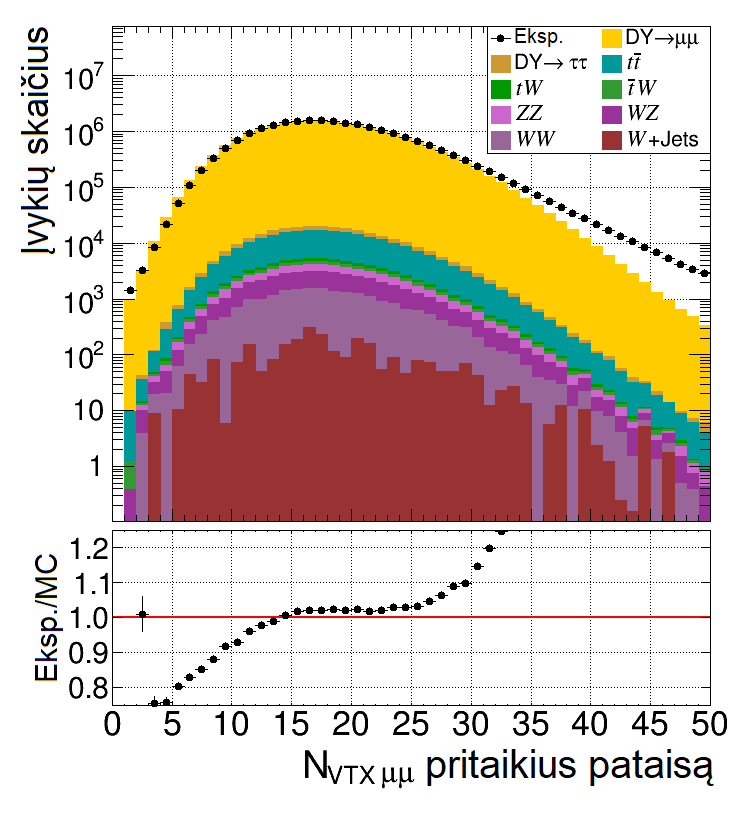
\includegraphics[width=0.48\textwidth]{Kursinis3/mumu_nVTX_after.png}
	\vspace{-0.5cm}
	\caption{\label{fig:PUba} Pirminių viršūnių skaičiaus pasiskirstymai atranką praėjusiuose įvykiuose prieš (kairėje)
		ir po (dešinėje) protonų susidūrimų tankio pataisos pritaikymo.
		Juodi taškai vaizduoja CMS detektoriumi išmatuotą, o spalvoti stulpeliai -- modeliuotus pasiskirstymus \cite{MAk2}.}
	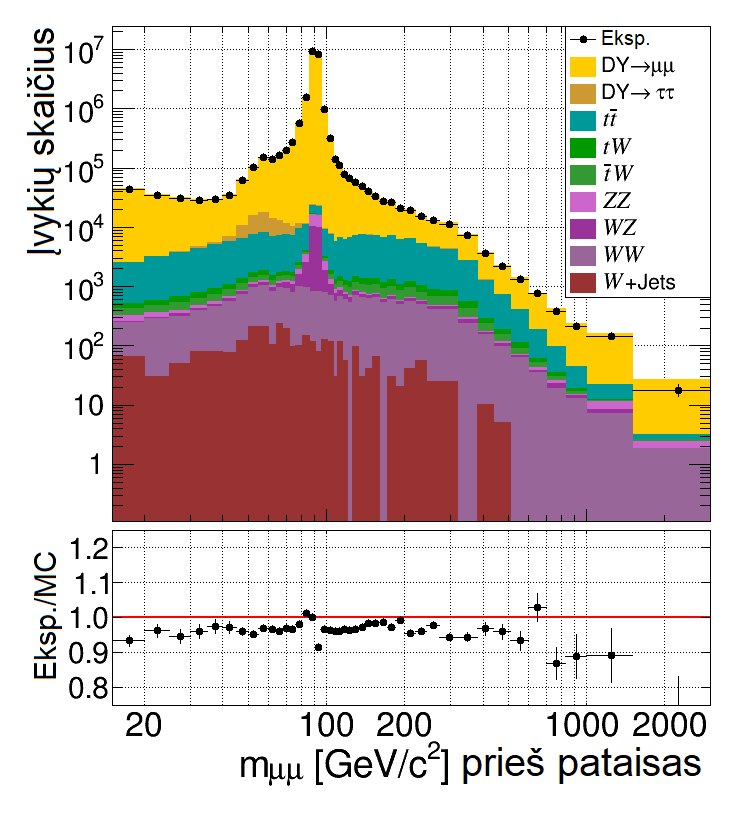
\includegraphics[width=0.48\textwidth]{Kursinis3/mumu_mass_before.png}
	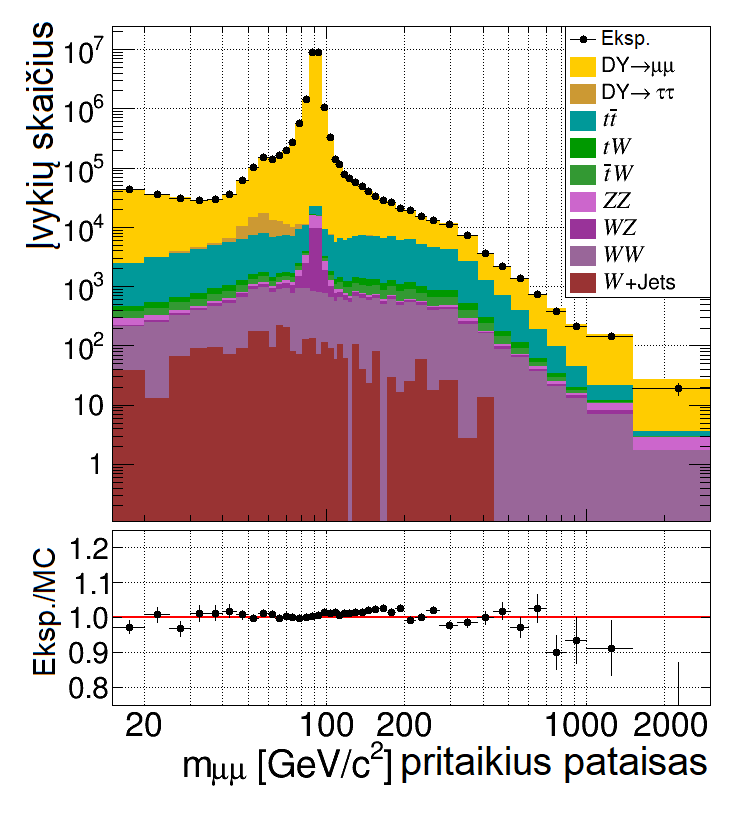
\includegraphics[width=0.48\textwidth]{Kursinis3/mumu_mass_afterSF.png}
	\vspace{-0.5cm}
	\caption{\label{fig:invMba} Miuonų porų invariantinės masės pasiskirstymai prieš ir po miuonų impulso matavimo skalės
	bei efektyvumo pataisų pritaikymo.}
\end{figure}

Matavimo ir modeliavimo rezultatų nesutapimą gali nulemti ne tik modeliavimo trūkumai, bet ir neidealios eksperimentinės sąlygos
arba eksperimentatorių klaidos.
Leptonų poros spartos pasiskirstymus paveikė dvi aplinkybės, į kurias buvo bandoma atsižvelgti pritaikant dar dvi pataisas.
Viena pataisa buvo skirta ištaisyti protonų susidūrimo vietos $z$ koordinatės ($z$ ašis eina išilgai protonų
spindulio lėkimo krypties detektoriaus centre) nesutapimą tarp matavimo ir modeliavimo.
Tai padėjo sumažinti matavimo ir modeliavimo santykio pasiskirstymuose buvusius asimetriškumus tarp teigiamų ir neigiamų leptonų
poros spartos verčių.
Antroji pataisa buvo reikalinga todėl, kad eksperimento duomenų registravimo laikotarpiu buvo susidurta su problema,
kai dėl laiko matavimo netikslumo trigerio suveikimas kartais buvo priskiriamas ne tam įvykiui, kuris iš tikrųjų jį aktyvavo, o
ankstesniam.
Dėl šio efekto dalis įdomių įvykių, kuriuose sukurtos dalelės turėjo dideles pseudospartos vertes ($|\eta|>2$) liko neįrašyti.
Imituoti šiam pernelyg ankstyvo trigerio suveikimo efektui buvo pritaikyta pataisa, kuri priskirdavo įvykiams
svorius pagal tai, kiek ir kokių įvykyje užregistruotų objektų patenka į didelių pseudospartų sritį.
Ši pataisa turėjo įtakos ir leptonų poros spartos pasiskirstymui.
Ji padėjo sumažinti modeliuotų įvykių skaičių prie didesnių spartos modulio verčių.
Tipinės pataisos vertės vienam įvykiui siekė apie $0.98$ ir mažiau, jeigu jame buvo užfiksuota objektų, kurių $|\eta|>2$.
Taip modeliuotas rezultatas buvo priartintas prie išmatuotojo.
\ref{fig:rapiba}~pav.\ pavaizduoti leptonų poros spartos pasiskirstymai prieš ir po abiejų minėtų pataisų pritaikymo.

\begin{figure}[b!]
	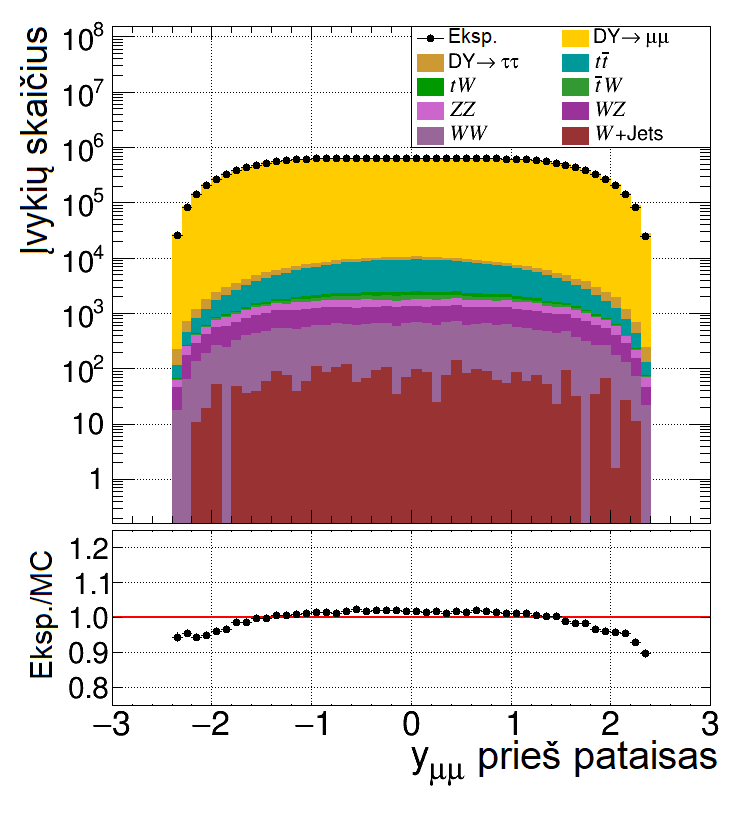
\includegraphics[width=0.48\textwidth]{Kursinis3/mumu_rapi_beforePVz.png}
	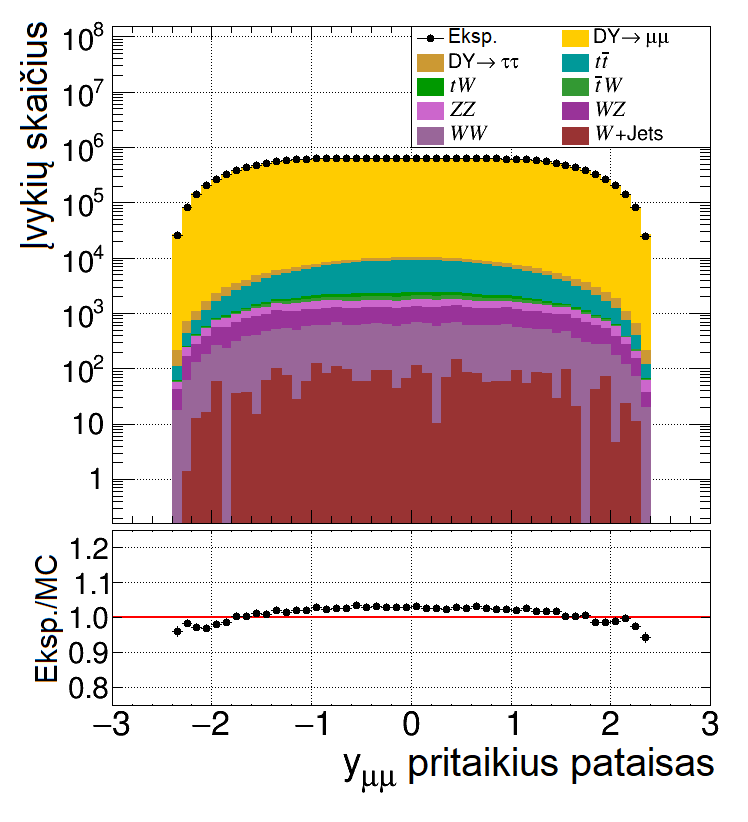
\includegraphics[width=0.48\textwidth]{Kursinis3/mumu_rapi_after.png}
	\vspace{-0.5cm}
	\caption{\label{fig:rapiba} Miuonų porų spartos pasiskirstymai prieš ir po pirminės viršūnės $z$ koordinatės bei per ankstaus
	trigerio suveikimo pataisų pritaikymo \cite{MAk2}.}
\end{figure}

\subsection{Triukšmo įvykių skaičiaus įvertinimas}\label{sec:FRresults}

Drell-Yan proceso triukšmo įvykių skaičius, susijęs su $\DYtau$, $t\bar{t}\,$, $WW$, $tW$, $\bar{t}W$ procesais buvo įvertintas
$\emu$ metodu ankstesniame darbe \cite{MAk2}.
Šie triukšmo įvykiai sudaro $1.06\%$ visų $\mu\mu$ įvykių.
Sisteminė $\emu$ metodo įverčio paklaida buvo įvertinta kaip skirtumo tarp modeliuoto ir $\emu$ metodo įverčio modulis, pagal
CMS statistikos komiteto rekomendacijas.
Invariantinės masės histogramų, kai naudojami vien modeliuoti įverčiai ir kai naudojamas $\emu$ metodas palyginimas pateikiamas
\ref{fig:MassMCemu}~pav.
Modeliuotų $\mu\mu$ triukšmo įvykių skaičius lygus $250500$, o įvertinus $\mu\mu$ triukšmo įvykių skaičių  $e\mu$ metodu
gauta $241105$ įvykių.
Lyginant su modeliavimu, $\emu$ metodas visoje tirtoje invariantinės masės srityje susumuotą triukšmo įvykių skaičių
sumažino maždaug $4$-ais procentais.
Abiejuose pateikiamuose grafikuose naudojami modeliuoti $\WZ$, $\ZZ$, $\WJets$ ir $\QCD$ procesų įverčiai.
Verta atkreipti dėmesį, kad modeliuoti $\WJets$ ir $\QCD$ procesų įverčiai turi netolydžius invariantinės masės pasiskirstymus:
įvykių skaičiaus skirtumai tarp gretimų histogramos stulpelių vietomis skiriasi dešimtimis kartų, daug stulpelių yra tušti
net žemų masių srityse (ypač $\QCD$ atveju).
Tai rodo prastą šių dviejų procesų modeliavimo kokybę.
$\QCD$ ir $\WJets$, lyginant su kitais Drell-Yan triukšmo procesais turi labai didelį reakcijos skerspjūvį, tačiau artimą
nuliui tikimybę praeiti Drell-Yan proceso atranką.
Sumodeliavus tiek su šiais procesais susijusių įvykių, kiek leidžia turimi skaičiavimo resursai ($2.8\cdot10^8$ $\QCD$ ir
$6.3\cdot10^8$ $\WJets$ įvykių), iš jų Drell-Yan proceso atranką praeina vos $40$ $\QCD$ ir $1288$ $\WJets$ įvykiai.
Dėl didelio reakcijos skerspjūvio šiems įvykiams priskiriami dideli svoriai, kurių vertės siekia net iki kelių tūkstančių:
sunormavus įvykius pagal išmatuotą integruotąjį šviesį buvo gauta $1673\pm1498$ $\QCD$ ir $2704pm200$ $\WJets$ įvykių. 
Tai paaiškina pasiskirstymuose matomus netolydumus ir yra pagrindinė priežastis, kodėl šių triukšmų indėlį reikia įvertinti
matavimu grįstais metodais.

\begin{figure}[b!]
	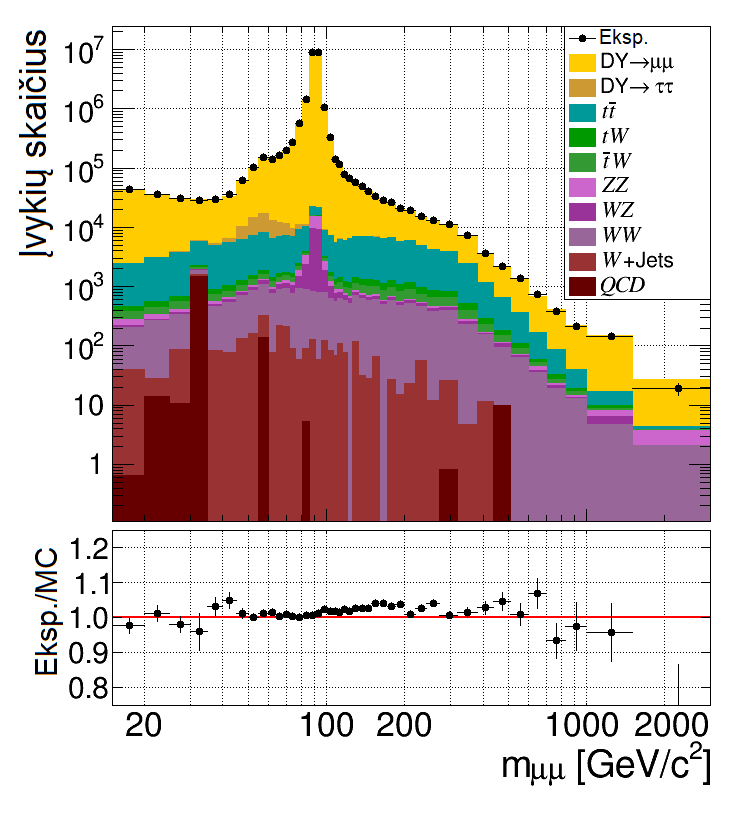
\includegraphics[width=0.49\textwidth]{Kursinis3/mumu_mass_after_wQCD.png}
	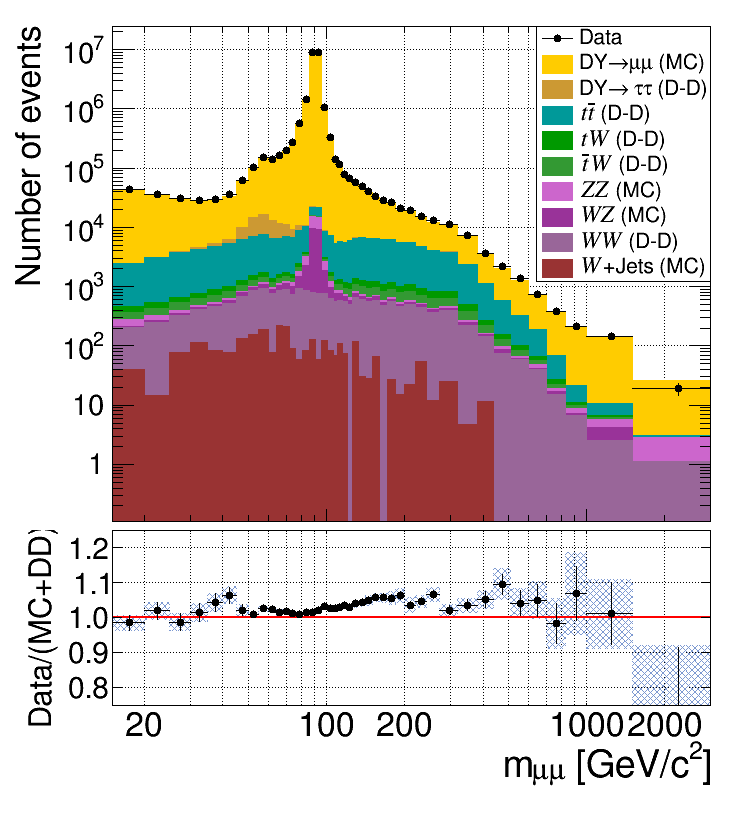
\includegraphics[width=0.49\textwidth]{Kursinis3/mumu_mass_wEMuEst.png}
	\vspace{-0.5cm}
	\caption{\label{fig:MassMCemu}
		Miuonų poros invariantinės masės pasiskirstymai pritaikius visas pataisas.
		Juodi taškai vaizduoja CMS detektoriumi išmatuotus pasiskirstymus, o spalvoti stulpeliai -- modeliuotus (kairėje)
		arba $\emu$ metodu įvertintus (dešinėje) įvykius.
		Eksperimento ir įverčio santykio grafike esančios mėlynos juostos vaizduoja sumines paklaidas.}
\end{figure}

Įvykiai klaidingo atpažinimo tikimybei įvertinti buvo atrenkami pagal \ref{table:FR}~lentelėje nurodytus atrankos kriterijus.
Drell-Yan signalo atrankoje naudoti vieno miuono trigeriai šiuo atveju buvo netinkami, nes juose yra užkoduotas ir miuono trajektorijos
izoliuotumo reikalavimas, kuris šiuo atveju buvo nereikalingas.
Dėl šios priežasties buvo pasirinktas kitas vieno miuono trigeris, kuris aktyvuojamas, kai aptinkamas miuonas su skersiniu impulsu,
viršijančiu $50$~GeV. Šis trigeris neatsižvelgia į miuono izoliuotumą.
Dėl pasikeitusio trigerio buvo naudojami ir kitokie kinematiniai reikalavimai: atrenkami miuonai su $\pT>52$~GeV.
Miuonams buvo taikomas tas pats Drell-Yan signalo atrankoje naudotas \ttt{TightID} reikalavimas.
Reikalavimai miuono krūviui ar įvykyje užregistruotų miuonų skaičiui nebuvo taikomi.
Klaidingo atpažinimo tikimybė buvo įvertinta pagal \eqref{eq:realfake} formulę keliose skirtingose miuono skersinio impulso ir
pseudospartos srityse ($f_{\mathrm{Signal} \, | \, \mathrm{Jet}}$ yra funkcija nuo $\pT$ ir $\eta$).

\begin{table}[t!]
	\begin{tabular}{|c|c|}
		\hline
		\textbf{Signalo sritis} & \textbf{Kontrolinė sritis} \\
		\hline\hline
		\multicolumn{2}{|c|}{Aukšto lygio trigeris \ttt{Mu\_50}} \\
		\hline
		\multicolumn{2}{|c|}{$\pT>52$~GeV} \\
		\hline
		\multicolumn{2}{|c|}{$|\eta|<2.4$} \\
		\hline
		\multicolumn{2}{|c|}{\ttt{TightID} reikalavimai} \\
		\hline
		$I_{\mathrm{PF}}^{\mathrm{rel.}} < 0.15$ & $I_{\mathrm{PF}}^{\mathrm{rel.}} > 0.15$ \\
		\hline
	\end{tabular}
	\caption{\label{table:FR} Naudoti miuonų atrankos kriterijai signalo ir kontrolinei sritims. Visi kriterijai, išskyrus vieną
	abiem sritims yra vienodi.}
\end{table}

\begin{figure}[b!]
	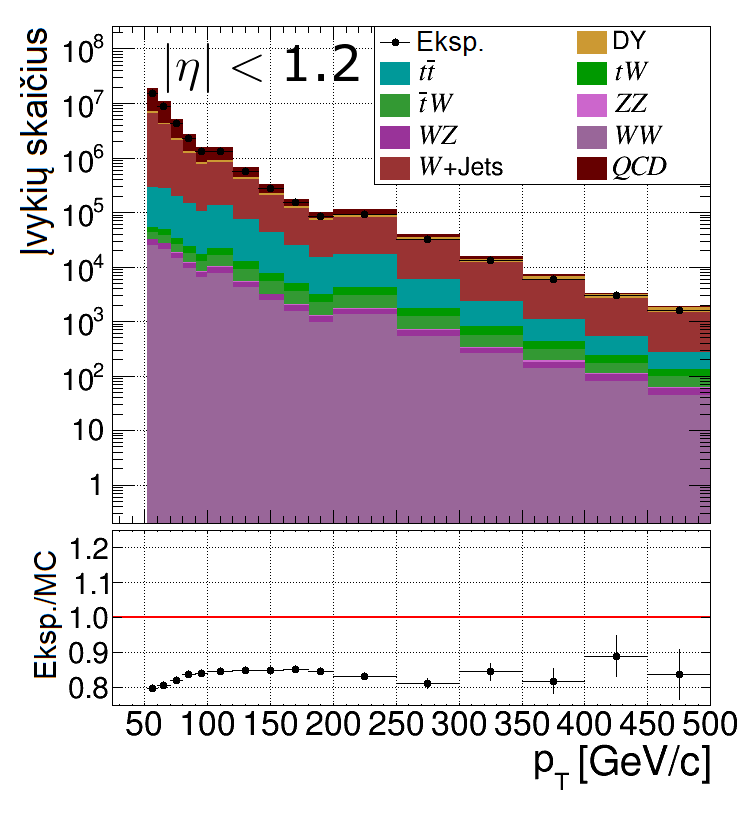
\includegraphics[width=0.48\textwidth]{Kursinis3/FRest_pT_deno_barrel.png}
	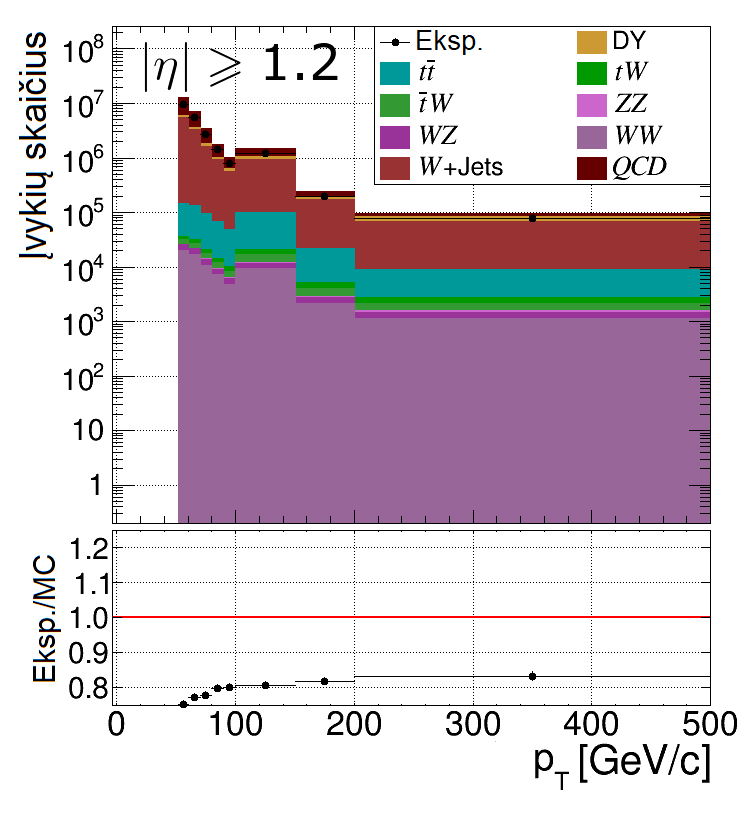
\includegraphics[width=0.48\textwidth]{Kursinis3/FRest_pT_deno_endcap.png}
	\vspace{-0.5cm}
	\caption{\label{fig:jet_pT_before}
		Klaidingo atpažinimo tikimybės įvertinimui atliktą įvykių atranką praėjusių miuonų kandidatų skersinių impulsų
		pasiskirstymai, kai miuonas pataiko į detektoriaus cilindrinę (kairėje) ir antgalio (dešinėje) dalį.
		Dėl nepakankamai tikslaus modeliavimo, jo sutapimas su eksperimento rezultatu yra prastas.}
\end{figure}

\begin{figure}[p!]
	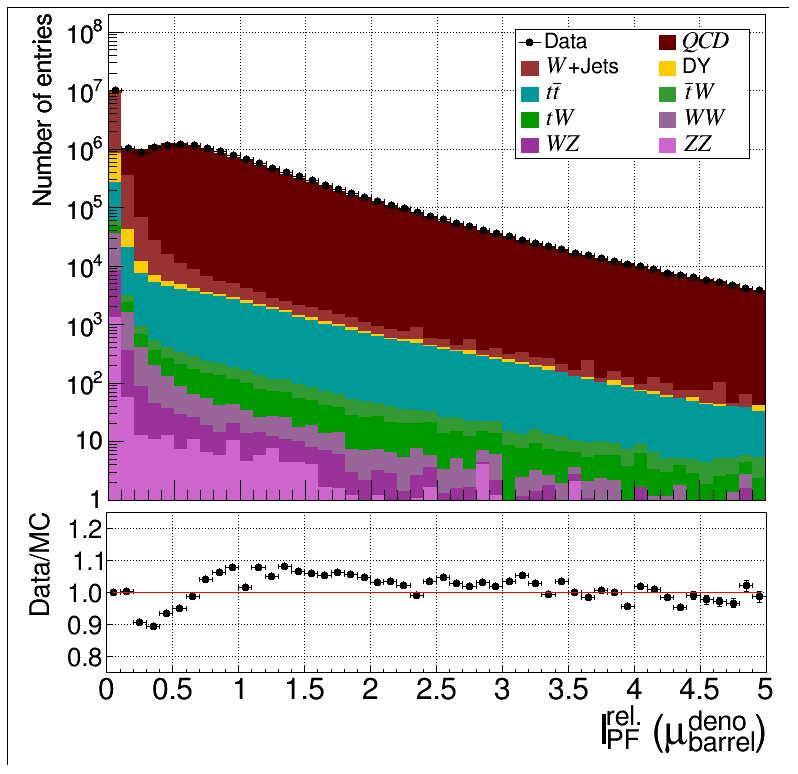
\includegraphics[width=0.45\textwidth]{Kursinis3/TFit_DB_50to70.png}
	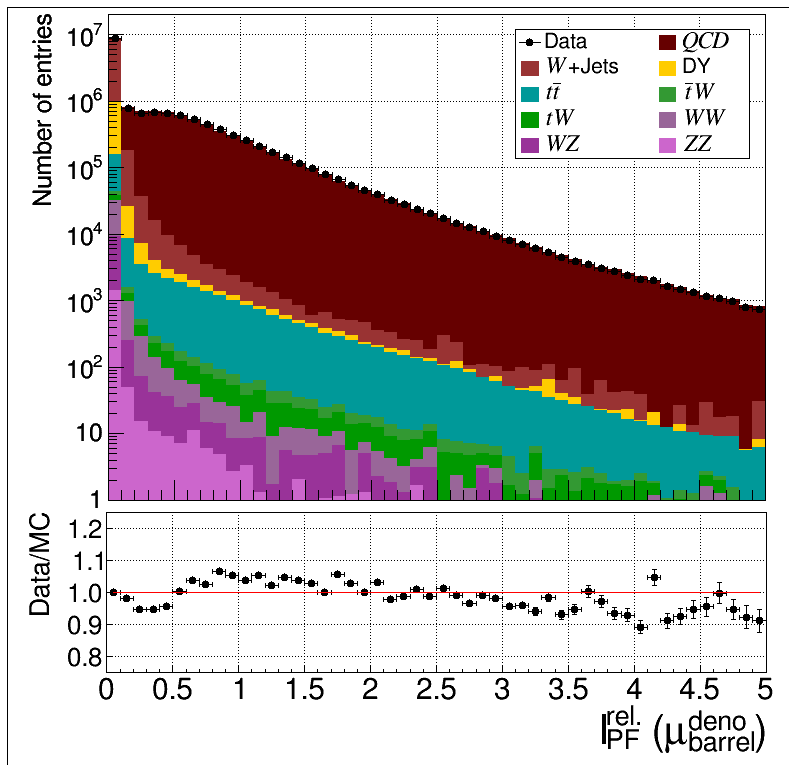
\includegraphics[width=0.45\textwidth]{Kursinis3/TFit_DE_50to70.png}
	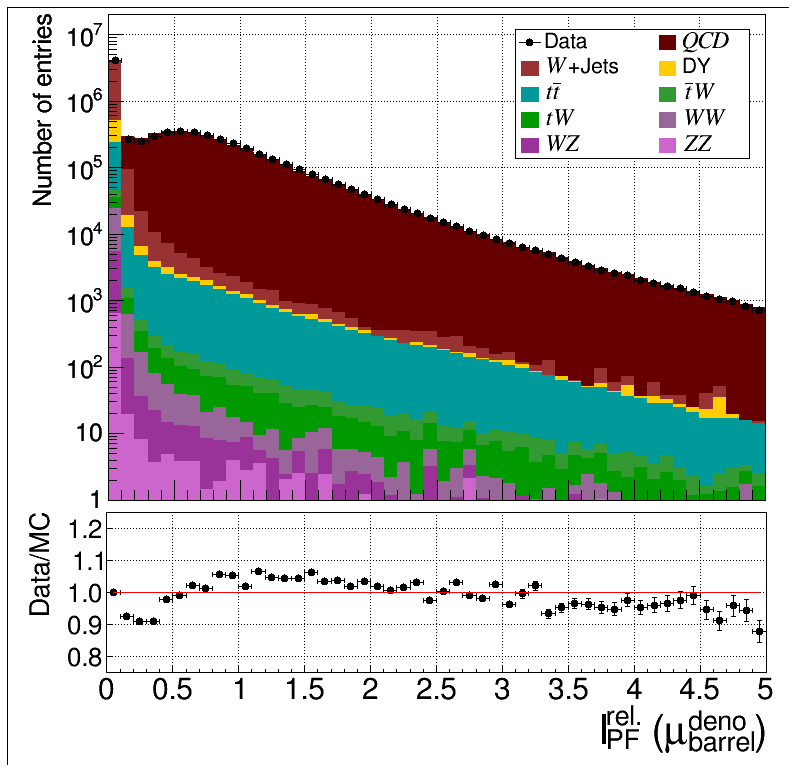
\includegraphics[width=0.45\textwidth]{Kursinis3/TFit_DB_70to100.png}
	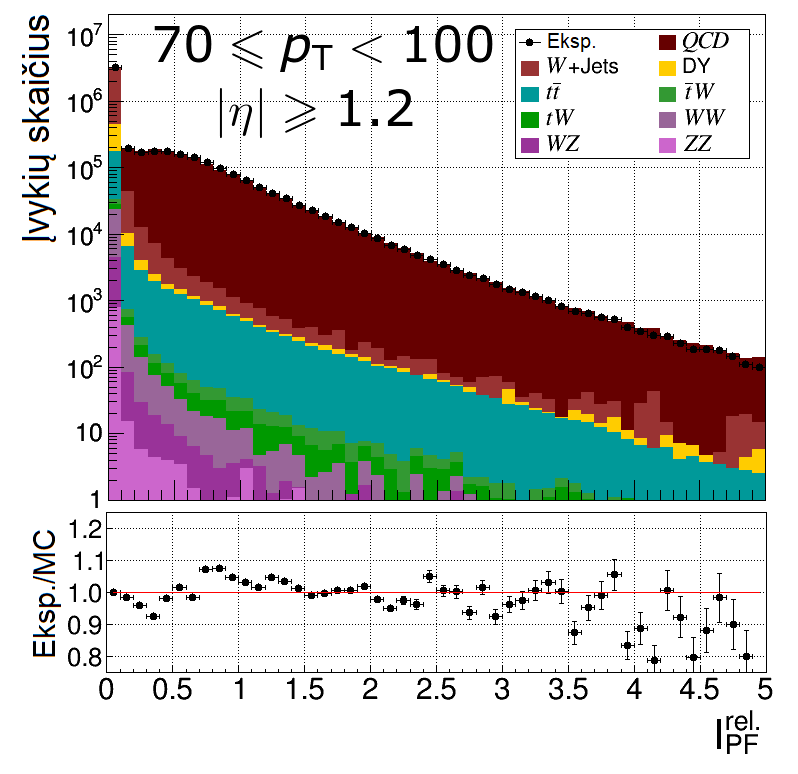
\includegraphics[width=0.45\textwidth]{Kursinis3/TFit_DE_70to100.png}
	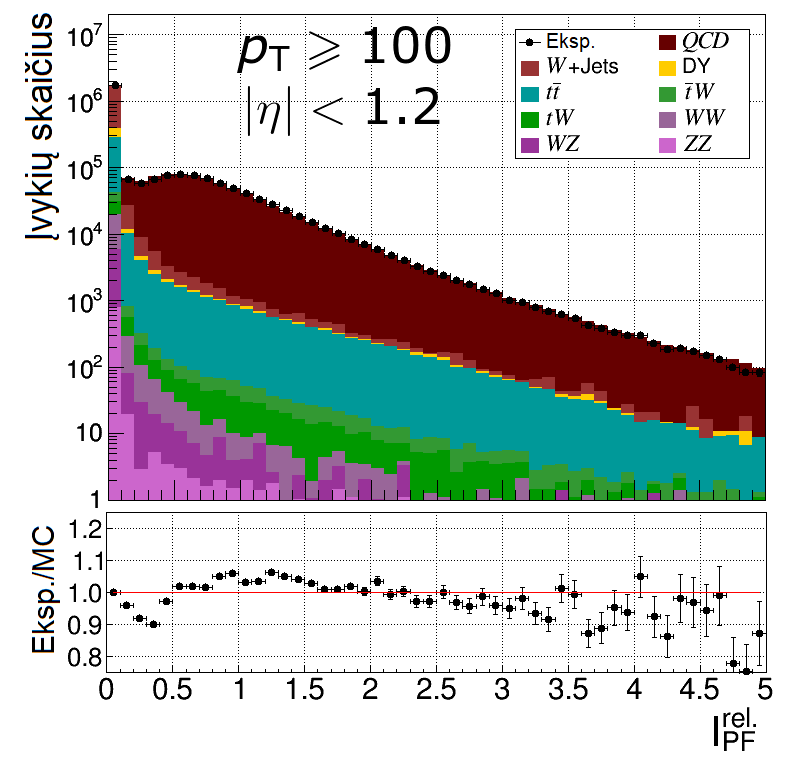
\includegraphics[width=0.45\textwidth]{Kursinis3/TFit_DB_100to500.png}
	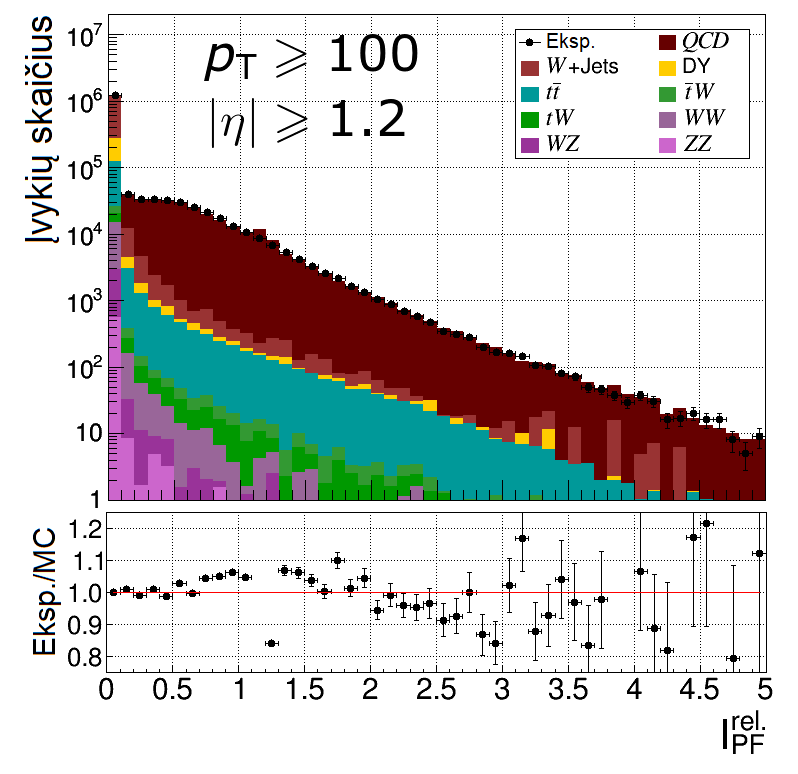
\includegraphics[width=0.45\textwidth]{Kursinis3/TFit_DE_100to500.png}
	\vspace{-0.2cm}
	\caption{\label{fig:templateFit}
		Eksperimentiniai miuono trajektorijos izoliuotumo pasiskirstymai detektoriaus cilindrinėje (kairėje)
		ir  antgalių (dešinėje) dalyse, bei prie jų pritaikyti modeliuoti šablonai.
		Iš viršaus į apačią pavaizduoti pasiskirstimai miuonų kandidatams, kurių $\pT\in(52, 70)$~GeV,
		$\pT\in[70, 100)$~GeV ir $\pT\in[100, 500)$~GeV.}
\end{figure}

\ref{fig:jet_pT_before}~pav.\ pavaizduoti atranką praėjusių miuonų skersinio impulso pasiskirstymai.
Dėl nepakankamai tikslaus modeliavimo nesutapimas tarp eksperimento ir modeliavimo siekia $20\%$.
Dėl šios priežasties buvo laikoma, jog klaidingo atpažinimo tikimybės įvertinimas naudojant santykio metodą gali būti
nepakankamai teisingas.
Kokybiškesnį įvertinimą buvo tikimasi gauti naudojant šablonų pritaikymo metodą.
Jis buvo atliekamas prie matavimo pritaikant modeliuotus miuono trajektorijos izoliuotumo pasiskirstymus.
Izoliuotumo pasiskirstymai buvo padalinti į šešias sritis: pirmiausia dalinama į dvi dalis pagal miuono pseudospartą
($|\eta|<1.2$ atitinka miuonus, pataikiusius į detektoriaus cilindrinę dalį, o $|\eta|\geqslant 1.2$ -- į antgalių segmentus)
bei į tris dalis pagal miuono skersinį impulsą ($\pT\in(52, 70)$~GeV, $\pT\in[70, 100)$~GeV ir $\pT\in[100, 500)$~GeV).
Prie išmatuotų izoliuotumo pasiskirstymų pritaikyti šablonai pavaizduoti \ref{fig:templateFit}~pav.
Iš šablonų pritaikymo gautos normavimo daugiklio vertės $\QCD$ pasiskirstymams siekė $0.72$-$0.75$ cilindrinėje detektoriaus
srityje ir $0.60$-$0.66$ antgalių srityje.
Šablonų pritaikymas pakoregavo modeliuotų pasiskirstymų normavimą taip, kad nesutapimas tarp matavimo ir modeliavimo
sumažėjo iki $5\%$.
Pernormuoti miuonų skersinio impulso pasiskirstymai pavaizduoti \ref{fig:jet_pT_after}~pav.
Klaidingo atpažinimo tikimybė buvo įvertinta skirtingose miuono skersinio impulso srityse bei dviejose pseudospartos srityse
(atitinkančiose detektoriaus cilindro ir antgalių segmentus) naudojantis \ref{eq:FR} formule.
Klaidingo atpažinimo tikimybės vertės, gautos naudojant santykio ir šablonų pritaikymo metodus, pavaizduotos \ref{fig:FR}~pav.
Šablonų pritaikymo metodu gautos klaidingo atpažinimo tikimybės vertės yra beveik $10\%$ didesnės, už įvertintas
santykio metodu.
Čiurkšlėms, pataikiusioms į cilindrinę detektoriaus dalį, klaidingo atpažinimo tikimybė kinta apytiksliai nuo $5\%$ iki $20\%$,
o pataikiusioms į detektoriaus antgalį ji yra vidutiniškai $2.5$ karto didesnė ir kinta
apytiksliai nuo $14\%$ iki $32\%$.

\begin{figure}[p!]
	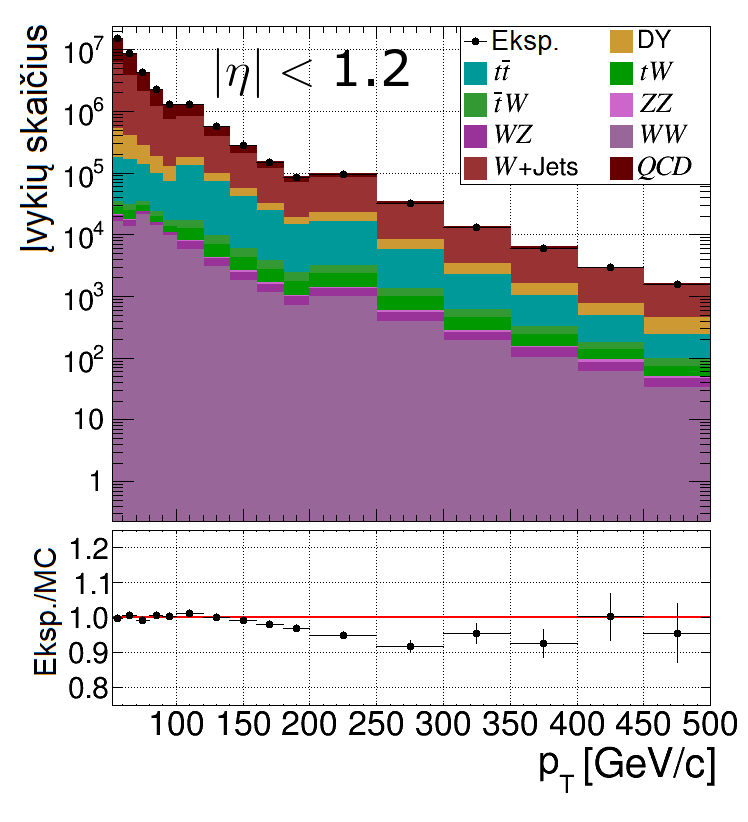
\includegraphics[width=0.48\textwidth]{Kursinis3/FRfit_pT_deno_barrel.png}
	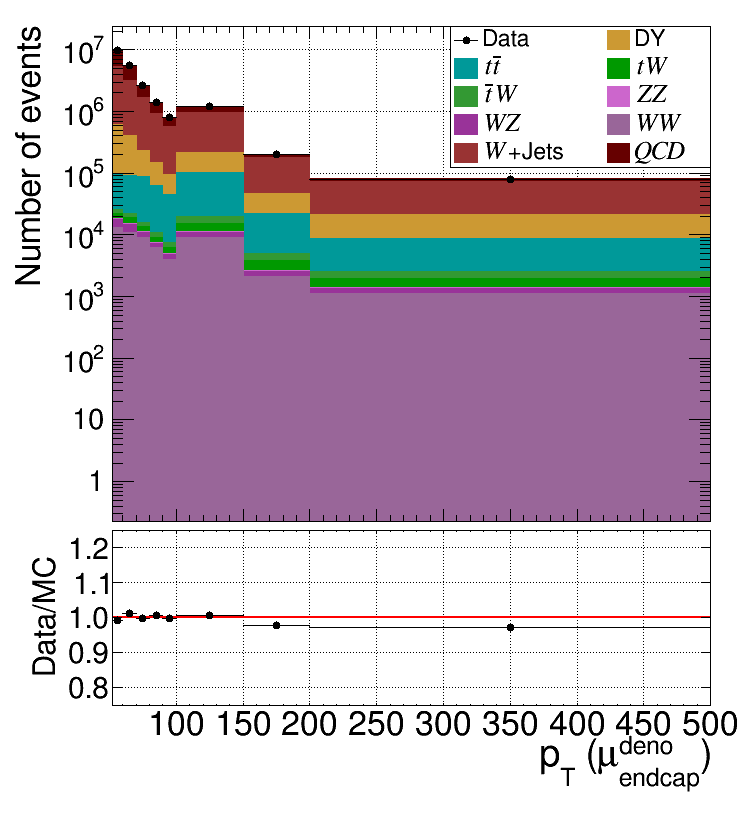
\includegraphics[width=0.48\textwidth]{Kursinis3/FRfit_pT_deno_endcap.png}
	\vspace{-0.4cm}
	\caption{\label{fig:jet_pT_after}
		Klaidingo atpažinimo tikimybės įvertinimui atliktą įvykių atranką praėjusių miuonų kandidatų skersinių impulsų
		pasiskirstymai, kai miuonas pataiko į detektoriaus cilindrinę (kairėje) ir antgalio (dešinėje) dalį.
		Šiuose grafikuose modeliuoti pasiskirstymai (parodyti \ref{fig:jet_pT_before}~pav.)\ yra pernormuoti, kad
		atitiktų iš šablonų pritaikymo gautas vertes.}
\end{figure}

\begin{figure}[p]
	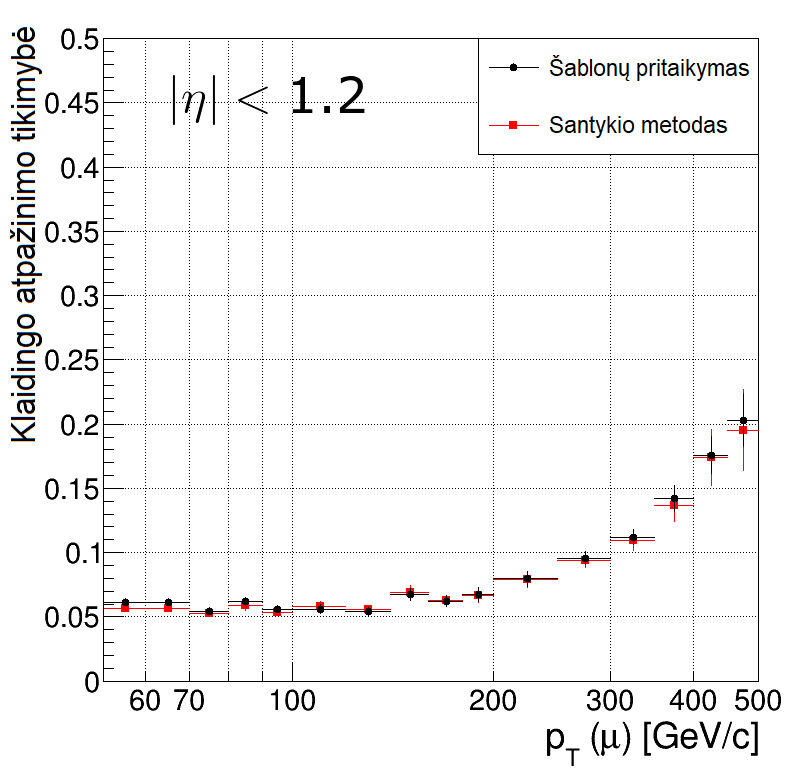
\includegraphics[width=0.48\textwidth]{Kursinis3/FR_barrel.png}
	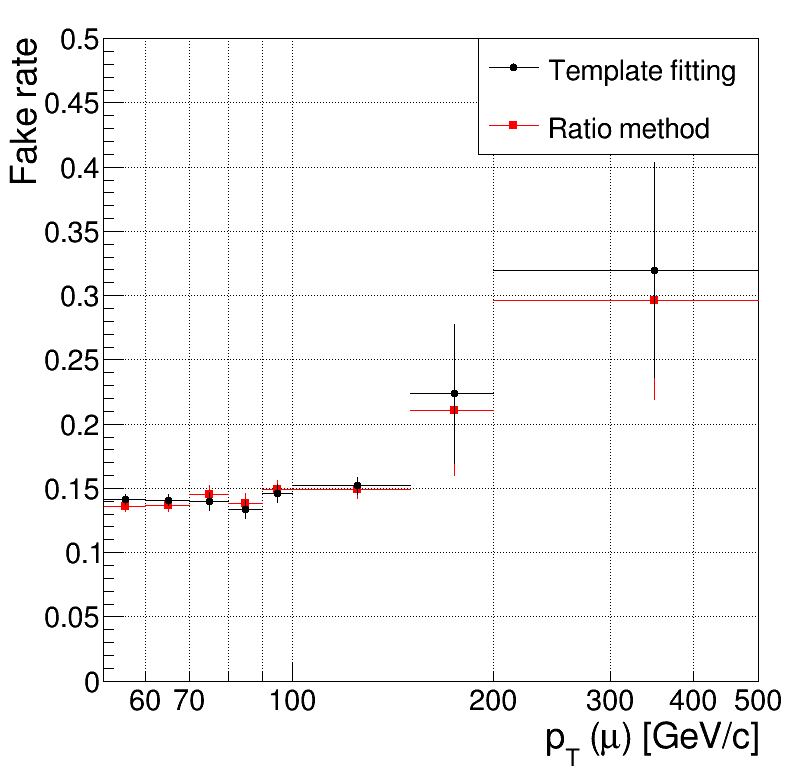
\includegraphics[width=0.48\textwidth]{Kursinis3/FR_endcap.png}
	\vspace{-0.3cm}
	\caption{\label{fig:FR}
		Apskaičiuota klaidingo atpažinimo tikimybė skirtingose skersinio impulso srityse.
		Kairėje pateiktas rezultatas trajektorijoms, einančioms per detektoriaus cilindrinę, o dešinėje -- per antgalių dalis.
		Skirtingos spalvos vaizduoja skirtingais metodais įvertintą tikimybę (žr.~legendą).}
\end{figure}

Apskaičiuota klaidingo atpažinimo tikimybė buvo panaudota įvertinant Drell-Yan proceso triukšmo įvykių skaičių, susijusį su
$\QCD$ ir $\WJets$ procesais.
Šių triukšmo įvykių skaičiaus įvertinimui buvo vykdoma atranka, kurios kriterijai nurodyti \ref{table:jetSelection}~lentelėje.
Praktiškai visi taikyti atrankos kriterijai buvo identiški Drell-Yan signalo atrankos kriterijams, nurodytiems
\ref{table:selection}~lentelėje, tačiau vienam arba dviems miuonams buvo taikomi invertuoti trajektorijos izoliuotumo
reikalavimai (atitinkamai $\WJets$ arba $\QCD$ atrankoje).
Taip pat šiuo atveju nebuvo naudojamas joks aukšto lygio trigeris (naudotas tik pirmo lygio vieno miuono trigeris, kuris
ir taip buvo naudojamas visoje atliktoje analizėje), nes, norint teisingai įvertinti triukšmo įvykių skaičių
svarbu, kad taikomi kinematiniai reikalavimai atitiktų naudojamus pagrindinėje analizėje.
To nebūtų įmanoma padaryti naudojant klaidingo atpažinimo tikimybės įvertinimui naudotą trigerį \ttt{Mu\_50},
o pagrindinės analizės trigeriai taip pat buvo netinkami dėl jau minėto reikalavimo miuonų izoliuotumui.
Smarkaus skaičiavimo laiko išaugimo dėl aukšto lygio trigerio nenaudojimo buvo išvengta iškart atmetant visus įvykius,
kuriuose nebuvo užfiksuota bent dviejų miuonų.

\begin{table}[b!]
	\begin{tabular}{|c|c|}
		\hline
		\textbf{$\WJets$ atranka} & \textbf{$\QCD$ atranka} \\
		\hline\hline
		\multicolumn{2}{|c|}{Trigeris: pirmo lygio \ttt{SingleMuon} trigeris, jokio aukšto lygio trigerio} \\
		\hline
		\multicolumn{2}{|c|}{$p_{\mathrm{T \, 1}} > 28$~GeV, $p_{\mathrm{T \, 2}} > 17$~GeV} \\
		\hline
		\multicolumn{2}{|c|}{$|\eta_1| < 2.4$, $|\eta_2| < 2.4$} \\
		\hline
		\multicolumn{2}{|c|}{\ttt{TightID} reikalavimai} \\
		\hline
		\multicolumn{2}{|c|}{\multirow{2}{37em}{\centering Pasirenkami 2 miuonai, kuriuos galima tiksliausiai suvesti į vieną
		pirminę viršūnę su $\chi^2<20$}} \\
		\multicolumn{2}{|c|}{} \\
		\hline
		\multicolumn{2}{|c|}{Priešingi elektriniai krūviai} \\
		\hline
		\multicolumn{2}{|c|}{Plokštuminis kampas $< \pi - 0.005$ rad} \\
		\hline
		\multirow{1}{22em}{\centering Vienam miuonui $I_{\mathrm{PF}}^{\mathrm{rel.}}<0.15$,
			kitam -- $I_{\mathrm{PF}}^{\mathrm{rel.}}\geqslant 0.15$} &
			\multirow{1}{15em}{\centering Abiems miuonams $I_{\mathrm{PF}}^{\mathrm{rel.}}\geqslant 0.15$} \\
		\hline
	\end{tabular}
	\caption{\label{table:jetSelection}Apibendrinti $\WJets$ ir $\QCD$ įvykių atrankos kriterijai. Indeksai $1$ ir $2$ žymi
	atitinkamai greitesnįjį ir lėtesnįjį miuoną. Šios dvi atrankos skiriasi tik vienu kriterijumi.}
\end{table}

$\QCD$ įvykių skaičius iš kontrolinės į signalo sritį buvo perkeliamas atranką praėjusiems įvykiams pritaikius svorinius
daugiklius, apskaičiuojamus pagal \ref{eq:FRapply} formulę.
\ref{fig:FR}~pav.\ pavaizduoti klaidingo atpažinimo tikimybės priklausomybės nuo skersinio impulso grafikai tampa
plokšti mažų skersinių impulsų srityse, todėl atranką praėjusiems miuono kandidatams su $\pT<52$~GeV, buvo pritaikomi
tokie patys svoriniai daugikliai, kaip ir kandidatams su $\pT=52$~GeV.
Sisteminė įverčio paklaida buvo įvertinta pagal \ref{eq:systUncFR} formulę.
\ref{fig:QCDselection}~pav.\ pateiktas atranką praėjusių į signalo sritį perkeltų miuonų porų pasiskirstymas.
Modeliavimas sufleruoja, kad tokią įvykių atranką praeina ne tik $\QCD$ proceso įvykiai, tačiau pašaliniai įvykiai
sudaro tik apie $25\%$ viso įvykių skaičiaus.
$\QCD$ įvykių skaičius buvo gautas iš eksperimento metu išmatuoto pasiskirstymo atėmus modeliuotus pasiskirstymus.
Įverčio rezultatas pavaizduotas \ref{fig:QCDest}~pav.
Įvertintas su $\QCD$ procesu susijusių Drell-Yan proceso triukšmo įvykių skaičius yra $2884\pm 54 \pm 383$:
$1.7$ karto daugiau, nei buvo įvertinta iš modeliavimo.

\begin{figure}[b!]
	\RawFloats
	\begin{minipage}{0.48\textwidth}
		\vspace{-0.8cm}
		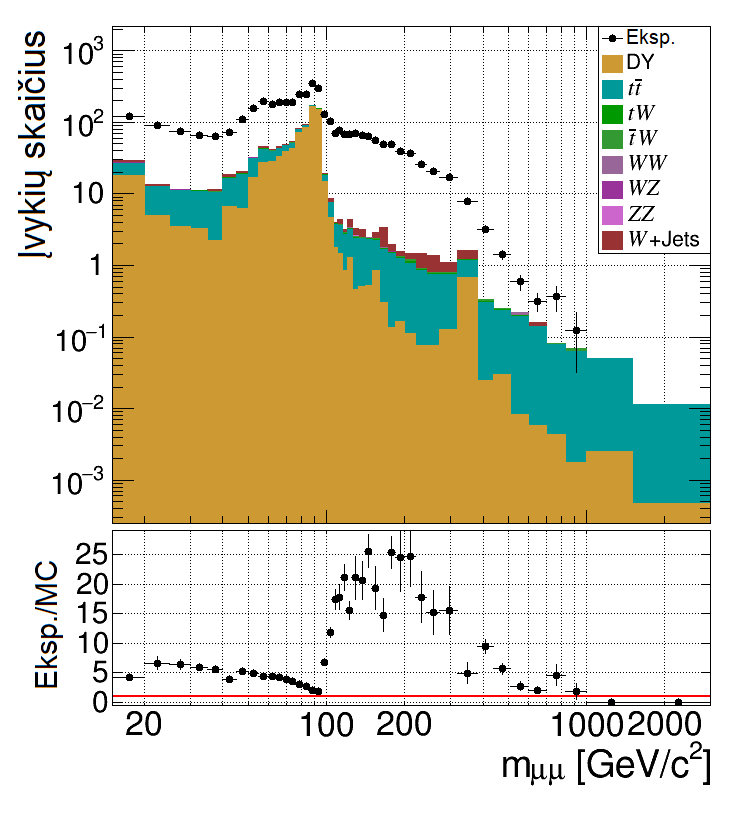
\includegraphics[width=0.95\textwidth]{Kursinis3/QCDest_subtract.png}
		\vspace{-0.53cm}
		\caption{\label{fig:QCDselection}
			$\QCD$ įvykių atranką praėjusių į signalo sritį perkeltų miuonų kandidatų porų invariantinės masės pasiskirstymas.
			Spalvotais stulpeliais pavaizduoti perkelti modeliuoti su $\QCD$ procesu nesusiję pasiskirstymai, kurie buvo atimami iš
			išmatuotojo pasiskirstymo.
		}
	\end{minipage}
	\hfill
	\begin{minipage}{0.48\textwidth}
		\vspace{-0.5cm}
		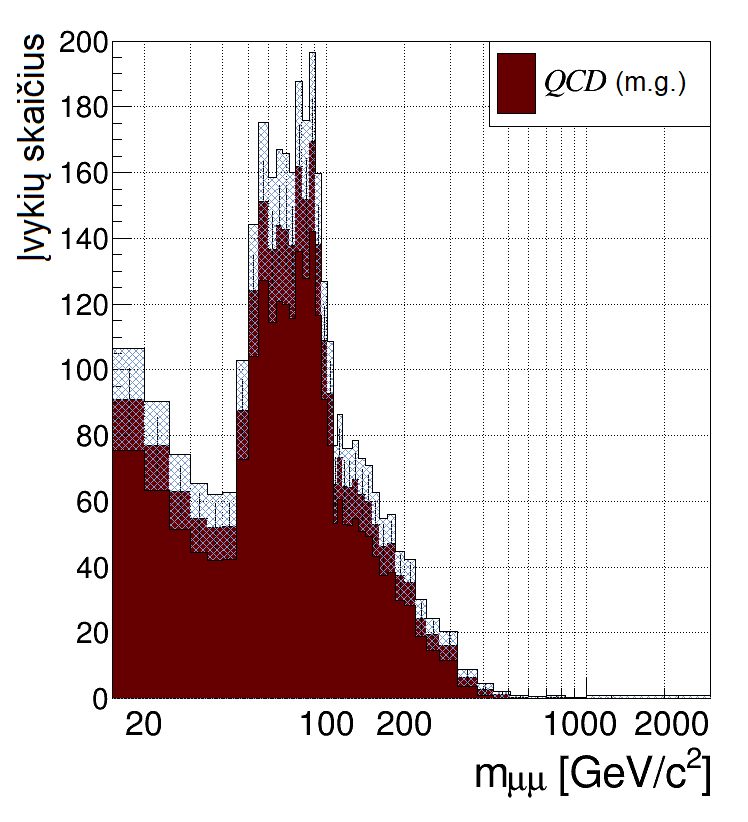
\includegraphics[width=0.95\textwidth]{Kursinis3/QCDest.png}
		\vspace{-0.35cm}
		\caption{\label{fig:QCDest}
			Klaidingo atpažinimo metodu įvertintas $\QCD$ proceso indėlis į Drell-Yan proceso atranką praeinančių miuonų
			porų invariantinės masės pasiskirstymą. Mėlynos juostos žymi sumines paklaidas. Legendoje esantis užrašas \ltq{m.g.}
			žymi faktą, jog tai yra matavimu grįstas įvertis.
		}
	\end{minipage}
	
	\begin{minipage}{0.48\textwidth}
		\vspace{-0.9cm}
		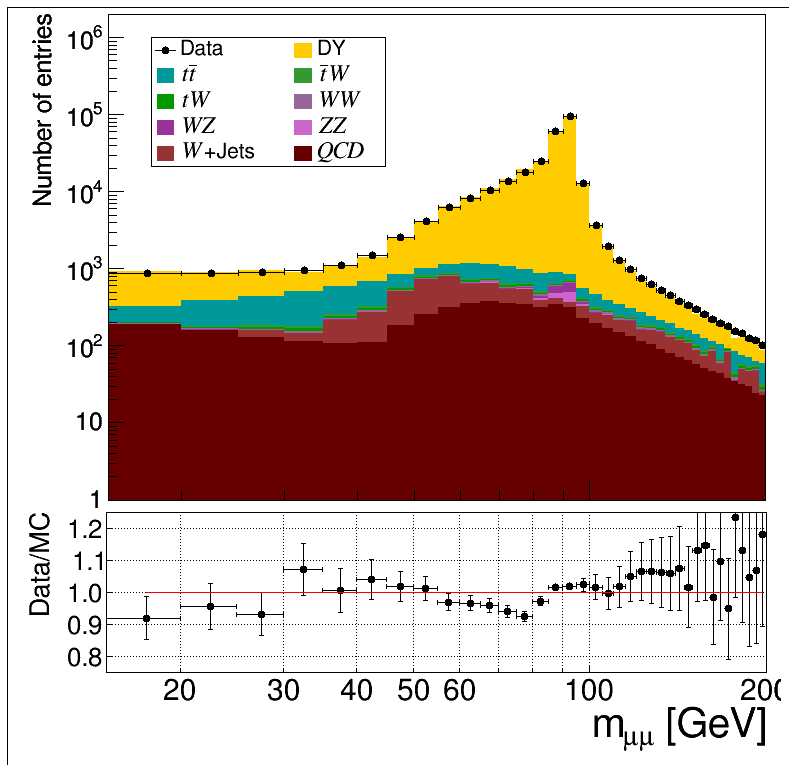
\includegraphics[width=0.98\textwidth]{Kursinis3/TFit_WJETS.png}
		\vspace{-0.4cm}
		\captionof{figure}{\label{fig:TFit_WJets}
			$\WJets$ įvykių atranką praėjusių į signalo sritį perkeltų miuonų kandidatų porų invariantinės masės pasiskirstymas
			bei prie jo pritaikyti skirtingų procesų šablonai.
		}
	\end{minipage}
	\hfill
	\begin{minipage}{0.48\textwidth}
		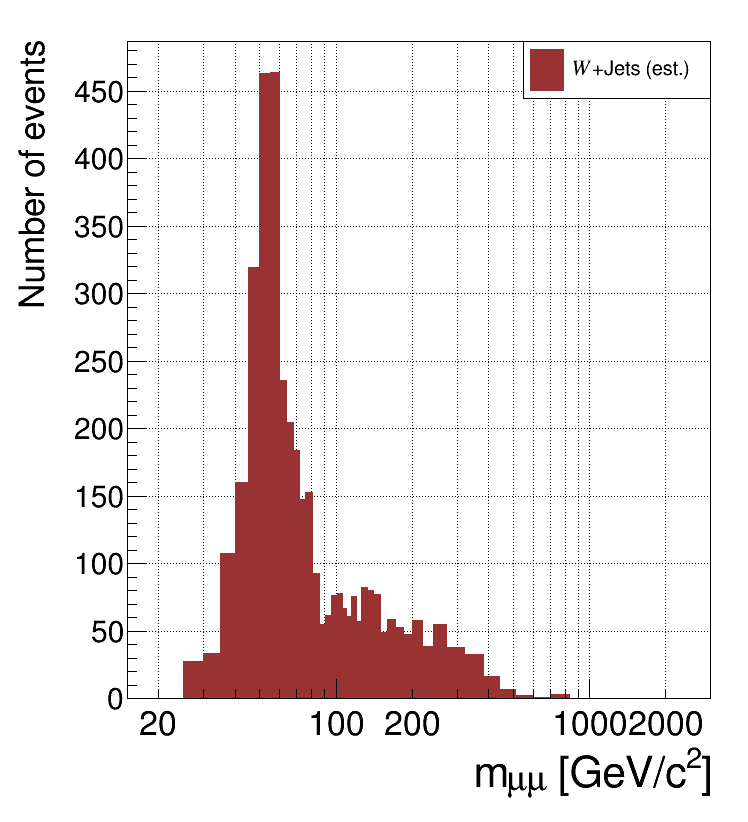
\includegraphics[width=0.9\textwidth]{Kursinis3/WJETSest.png}
		\vspace{-0.4cm}
		\captionof{figure}{\label{fig:WJetsEst}
			Klaidingo atpažinimo metodu įvertintas $\WJets$ proceso indėlis į Drell-Yan proceso atranką praeinančių miuonų
			porų invariantinės masės pasiskirstymą. Mėlynos juostos žymi sumines paklaidas, \ltq{m.g.} žymi, jog tai yra
			matavimu grįstas įvertis.
		}
	\end{minipage}
\end{figure}

$\WJets$ įvykių skaičius iš kontrolinės į signalo sritį buvo perkeliamas atranką praėjusiems įvykiams pritaikius svorinius
daugiklius pagal \ref{eq:FRapply} formulę.
Skirtingai nei $\QCD$ atranką, $\WJets$ atranką praeina didelė dalis pašalinių procesų: net $84.5\%$ visų įvykių yra
nesusiję su $\WJets$.
Modeliavimas sufleruoja, kad didžiausią indėlį į įvykių skaičių turi Drell-Yan ir $\ttbar$ procesai.
Tokiu atveju iš išmatuotojo pasiskirstymo atimti modeliuotą nėra tinkama procedūra, tad $\WJets$ pasiskirstymas buvo
gautas pasinaudojus šablonų pritaikymu.
Šiuo atveju šablonai buvo pritaikomi prie į signalo sritį perkeltų $\WJets$ atranką praėjusių miuonų porų invariantinės
masės pasiskirstymo.
$\WJets$ pasiskirstymo šablonas buvo gautas iš $\WJets$ atranką praėjusių vienodo krūvio miuonų pasiskirstymo,
kuris yra mažiau užterštas Drell-Yan proceso įvykiais.
Vienodo krūvio $\WJets$ pasiskirstymą galima naudoti kaip šabloną priešingo krūvio pasiskirstymui, nes čiurkšlėje įmanoma pagaminti
bet kokio krūvio miuoną ir vidutinė proceso kinematika nuo miuono krūvio neturėtų priklausyti.
Turėtų skirtis tik šių procesų tikimybės, tad tikimasi, jog pasiskirstymai bus apytiksliai vienodos formos, bet turės skirtingą
suintegruotą įvykių skaičių.
Iš modeliavimo buvo įvertinta, kad priešingo krūvio $\WJets$ įvykiai yra maždaug 3 kartus dažnesni, nei vienodo krūvio,
o jų pasiskirstymų forma yra panaši.
$\QCD$ proceso šablonas buvo gautas panaudojant klaidingo atpažinimo metodu įvertintą $\QCD$ pasiskirstymą.
Kitiems procesams buvo naudojami modeliuoti šablonai.

Šablonų pritaikymo rezultatas yra pateiktas \ref{fig:TFit_WJets}~pav.
Šablonų pritaikymas buvo atliktas tik iki $200$~GeV siekiančioje invariantinės masės srityje, nes prie aukštesnių
masių naudoti pasiskirstymai turi labai didelį statistinį išsibarstymą.
Gautas $\WJets$ įvykių skaičius yra lygus $3573 \pm 60 \pm 283$: $1.3$ karto daugiau, nei buvo įvertinta iš modeliavimo.
Tai yra $2.6$ kartų daugiau, nei vienodo krūvio įvykių skaičius.
Su $\WJets$ procesu susijusių triukšmo įvykių indėlio įvertis pavaizduotas \ref{fig:WJetsEst}~pav.
Lyginti klaidingo atpažinimo metodu gautus triukšmo įvykių pasiskirstymus su modeliuotais atitinkamų procesų įverčiais
nėra didelės prasmės, nes modeliuoti šių procesų pasiskirstymai yra smarkiai netolydūs dėl prastos statistikos.
Atkreiptinas dėmesys, jog tiek $\QCD$, tiek $\WJets$ įverčio sisteminės paklaidos yra ganėtinai didelės -- sudaro
reikšmingą dalį viso įvertinto įvykių skaičiaus ($13\%$ $\QCD$ atveju ir $7.4\%$ $\WJets$ atveju) bei kelis kartus
viršija statistines paklaidas ($7$ kartus $\QCD$ atveju ir $4.6$ karto $\WJets$ atveju).
Taip yra dėl to, jog įvertintas įvykių skaičius yra ganėtinai jautrus klaidingo atpažinimo tikimybės įvertinimo tikslumui
(ypatingai $\QCD$ įvykiams, kur klaidingo atpažinimo tikimybė taikoma du kartus).
Nepaisant to, toks įvertis yra gerokai kokybiškesnis už modeliuotą, kur vien statistinės paklaidos sudaro
didesnę dalį įvykių skaičiaus (net $90\%$ $\QCD$ atveju ir $8\%$ $\WJets$ atveju), o patys modeliuoti pasiskirstymai yra netolydūs.

Eksperimento metu išmatuoto Drell-Yan proceso atranką praėjusių miuonų porų invariantinių masių pasiskirstymo palyginimas
su susumuotais skirtingų procesų įverčiais, iš kurių tik $\WZ$ ir $\ZZ$ yra modeliuoti, yra pateiktas \ref{fig:MassFinal}~pav.
Lyginant su \ref{fig:MassMCemu}~pav.\ pateiktu grafiku, į kurį neįtraukti fizikinio objekto klaidingo atpažinimo metodo
įverčiai, sutapimas tarp matavimo ir įverčio pagerėjo $0.02\%$.
Nors pagerėjimas atrodo labai mažas, tačiau su čiurkšlėmis susiję atranką praėję įvykiai sudaro tik $0.03\%$ visų įvykių.
Beveik visi šie įvykiai prisideda prie matavimo ir įverčio sutapimo pagerėjimo, taigi fizikinio objekto klaidingo
atpažinimo metodo taikymas buvo naudingas.

\begin{figure}[H]
	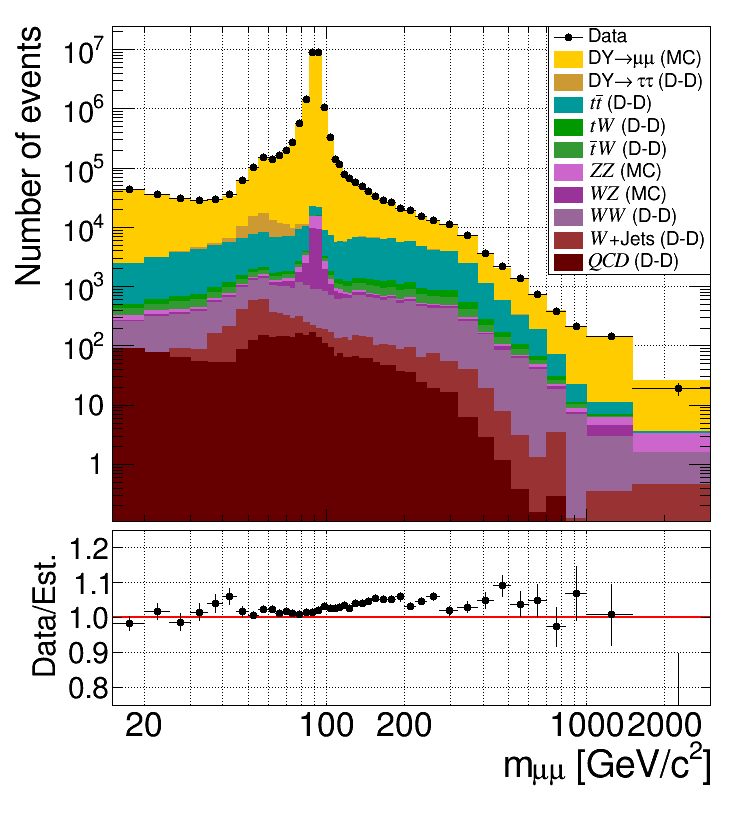
\includegraphics[width=0.5\textwidth]{Kursinis3/Mass_allEst.png}
	\vspace{-0.6cm}
	\caption{\label{fig:MassFinal}
		Eksperimento metu išmatuoto miuonų poros invariantinės masės pasiskirstymo palyginimas su matavimu grįstais
		skirtingų procesų indėlių įverčiais (pažymėta \ltq{m.g.}), išskyrus $\WZ$ ir $\ZZ$ procesų įverčius, kurie
		yra modeliuoti (pažymėta \ltq{MC}) Mėlynos juostos žymi sumines paklaidas.}
\end{figure}

\newpage
\section{Išvados}
\begin{enumerate}
	\item Šablonų pritaikymo metodas duoda geresnį modeliuotų pasiskirstymų sutapimą su eksperimento metu išmatuotais
	pasiskirstymais nei modeliuotų įvykių normavimas pagal išmatuotą integruotąjį šviesį, todėl manoma, kad šiuo metodu
	įvertinta tikimybė, kad čiurkšlė bus klaidingai atpažintai kaip izoliuotas miuonas, yra teisingesnė.
	\item Su čiurkšlėmis susijusių Drell-Yan proceso triukšmo įvykių skaičiaus įvertis yra labai jautrus
	fizikinio objekto klaidingo atpažinimo tikimybės įvertinimo tikslumui, todėl įverčio sisteminė paklaida yra didelė.
	\item Modeliuoti $\WJets$ ir $\QCD$ procesų įverčiai yra labai prastos kokybės dėl didelio šių procesų reakcijos
	skerspjūvio ir itin mažos tikimybės, kad su jais susiję įvykiai praeis Drell-Yan proceso atranką.
	\item Nors klaidingo atpažinimo metodu įvertintas $\WJets$ ir $\QCD$ procesų indėlis į miuonų poros invariantinės masės
	pasiskirstymą turi nemažus neapibrėžtumus, šio įverčio kokybė yra žymiai geresnė nei modeliuoto, tad fizikinio
	objekto klaidingo atpažinimo metodo taikymas buvo naudingas.
	\item Triukšmo įvykių skaičiaus įvertinimas fizikinio objekto klaidingo atpažinimo metodu pagerino eksperimento
	metu išmatuoto miuonų poros invariantinės masės pasiskirstymo sutapimą su skirtingų procesų įverčiais.
\end{enumerate}


\vspace{2cm}
\addcontentsline{toc}{section}{6 \hspace{0.1cm} Naudotos literatūros sąrašas}
\bibliography{KursinisDarbas}
\bibliographystyle{unsrt}

\section*{Santrauka}
\addcontentsline{toc}{section}{Santrauka}
Viena iš galimų reakcijų didelės energijos protonų susidūrimo metu yra kvarko-antikvarko anihiliacija, kurios
produktas -- leptono ir antileptono pora.
Tokia reakcija yra vadinama Drell-Yan procesu.
Eksperimentinis šio proceso tyrimas pasitarnauja protono sandaros aprašymo tikslinimui bei teorinių modelių testavimui.
Tirdami Drell-Yan procesą eksperimentatoriai ieško leptono-antileptono porų, tačiau jos gali susidaryti ne vien
Drell-Yan proceso metu.
Tokie pašaliniai įvykiai vadinami triukšmo įvykiais ir į jų indėlį svarbu atsižvelgti.
Galimi ir tokie triukšmo įvykiai, kuriuose susidariusios hadronų čiurkšlės yra klaidingai atpažįstamos kaip leptonai.

Šiame darbe pristatomas Drell-Yan proceso triukšmo įvykių skaičiaus įvertinimas fizikinio objekto klaidingo
atpažinimo metodu.
Darbas buvo atliktas analizuojant CERN CMS eksperimento 2016 metais užregistruotus
$13$~TeV energijos protonų susidūrimų duomenis, atitinkančius $35.9$~\invfb integruotąjį šviesį.
Duomenų interpretavimui buvo pasitelkiami CMS kolektyvo paruošti modeliuoti protonų susidūrimų duomenų rinkiniai.
Drell-Yan proceso įvykių atranką praėjusiems miuonams buvo pritaikytos skersinio impulso matavimo skalės pataisos.
Modeliuotiems įvykiams buvo pritaikytas rinkinys pataisų, įskaitančių įvairius neatitikimus tarp eksperimento
ir modeliavimo sąlygų.

Įvykdžius į Drell-Yan procesą panašių įvykių atranką buvo bandoma nustatyti, koks yra triukšmo įvykių, kuriuose
viena ar kelios čiurkšlės buvo klaidingai atpažintos kaip miuonai, skaičius.
Buvo įvertinta čiurkšlės klaidingo atpažinimo izoliuotu miuonu tikimybė.
Šios tikimybės vertės buvo panaudotos įvertinant, kiek $\WJets$ (vienos čiurkšlės) ir $\QCD$ (kelių čiurkšlių)
įvykių galėjo praeiti Drell-Yan proceso įvykių atranką bei koks šių procesų indėlis į eksperimento metu
išmatuotą miuonų poros invariantinės masės pasiskirstymą.
Nustatyta, jog su čiurkšlėmis susiję įvykiai sudaro $0.03\%$ visų Drell-Yan proceso atranką praėjusių įvykių.

\end{document}